\documentclass[10pt,mathserif]{beamer}

\usepackage{graphicx,amsmath,amssymb,tikz,psfrag,subfigure,cancel,mathabx}

\input defs.tex

%% formatting

\mode<presentation>
{
\usetheme{default}
}
\setbeamertemplate{navigation symbols}{}
\usecolortheme[rgb={0,0,0}]{structure}
\setbeamertemplate{itemize subitem}{--}
\setbeamertemplate{frametitle} {
	\begin{center}
	  {\large\bf \insertframetitle}
	\end{center}
}

\AtBeginSection[] 
{ 
	\begin{frame}<beamer> 
		\frametitle{Outline} 
		\tableofcontents[currentsection,currentsubsection] 
	\end{frame} 
} 

%% begin presentation

\title{\large \bfseries Probabilistic Graphical Models}

\author{Jiali Lin\\[3ex]
Virginia Tech}

\date{\today}

\begin{document}

\frame{
\thispagestyle{empty}
\titlepage
}

\section{Directed graphical models}
\subsection{Directed graphical models}
\begin{frame}{Frame Title}
\begin{itemize}
    \item First order Markov chain
    \begin{equation}
        p(x_{1:T}) = p(x_1)\prod_{t=2}^Tp(x_t |x_{t-1})
    \end{equation}
    \begin{figure}[h]
    \centering
    \includegraphics[width=0.4\textwidth]{markovChain1xCropped}
    \end{figure}

    \item Second order Markov chain
    \begin{equation}
        p(x_{1:T}) = p(x_1)p(x_2)\prod_{t=3}^Tp(x_t |x_{t-1,t-2})
    \end{equation}
    
    \begin{figure}[h]
    \centering
    \includegraphics[width=0.4\textwidth]{markovChain2}
    \end{figure}
\end{itemize}  
\end{frame}

\begin{frame}{General DAGs}
\begin{itemize}
    \item If the graph is a DAG (directed acyclic graph), we can order nodes such that parents come before children. This is called a \textbf{topological ordering}.
    
    \item  \textbf{Ordered Markov property} is the assumption that a node only depends on its immediate parents, not on all predecessors in the ordering, i.e.,
    \begin{equation}
        x_{s} \bot x_{\text{pred($s$)\textbackslash pa}(s)}|x_{\text{pa}(s)}
    \end{equation}
    where $\text{pa($s$)}$ are the parents of node $s$, and $\text{pred($s$)}$ are the predecessors of node $s$ in the ordering. This is a natural generalization of the first-order Markov property from chains to general DAGs.
    
    \item Each node has a CPD $p(x_{\text{t}}|x_{\text{pa(t)}})$
    \begin{equation}
        p(x_{1:V}|G) = \prod_{t=1}^V p(x_{\text{t}}|x_{\text{pa}(t)})
    \end{equation}
\end{itemize}   
\end{frame}

\begin{frame}{Example}
\begin{figure}[h]
\centering
\subfigure[]{\includegraphics[width=20mm]{DAGfive}}
\subfigure[]{\includegraphics[width=20mm]{UGMfive}}
\caption{A simple DAG on 5 nodes, numbered in topological order. Node 1 is the root, nodes 4 and 5 are the leaves. (b) A simple undirected graph, with the following maximal cliques: $\{1, 2, 3\}, \{2, 3, 4\}, \{3, 5\}$.}
\end{figure}

\begin{equation}
    \begin{split}
        p(x_{1 : 5}) & = p(x_{1})p(x_{2}|x_{1})p(x_{3}|x_{1},\cancel{x_{2}})p(x_{4}|\cancel{x_{1}},x_{2},x_{3})p(x_{5}|\cancel{x_{1}},\cancel{x_{2}},x_{3},\cancel{x_4})\\
        & = p(x_{1})p(x_{2}|x_{1})p(x_{3}|x_{1})p(x_{4}|x_{2}, x_{3})p(x_{5}|x_{3})
    \end{split}
\end{equation} 
\end{frame}

\begin{frame}{More examples}
\begin{figure}[h]
\centering     %%% not \center
\subfigure[]{\includegraphics[width=25mm]{TAN}}
\subfigure[]{\includegraphics[width=25mm]{NBCsimple}}
\caption{(a) A naive Bayes classifier represented as a DGM. We assume there are $D = 4$ features, for simplicity. Shaded nodes are observed, unshaded nodes are hidden. (b) Tree-augmented naive Bayes classifier for $D = 4$ features. In general, the tree topology can change depending on the value of $y$.}
\end{figure}        

Naive Bayes classifiers
\begin{equation}
    p(y,x) = p(y) \prod_{j=1}^D p(x_j|y)
\end{equation}

Tree-augmented naive Bayes:
\begin{equation}
    p(y,x) = p(y) \prod_{j=1}^D p(x_j|x_{\text{pa}(j)},y)
\end{equation} 
\end{frame}

\begin{frame}{More examples}
\begin{figure}[h]
\centering
\includegraphics[width=0.3\textwidth]{ldsDGM}
\caption{A first-order HMM.}
\end{figure}

Hidden Markov Models (HMMs)
\begin{equation}
    \begin{split}
        p(x_{1:T} , z_{1:T} ) & = p(z_{1:T} )p(x_{1:T} |z_{1:T} )\\
        & = \bigg[p(z_1)\prod_{t=2}^t p(z_t |z_{t-1})\bigg]\bigg[ \prod_{t=1}^t p(x_t |z_t )\bigg]
    \end{split}
\end{equation}

\begin{itemize}
    \item  Transition model $p(z_t = j|z_{t-1} = i) = A(i,j)$.
    \item  Discrete emission model $p(x_t = j|z_t = i) = B(i,j)$.
    \item  Gaussian emission model $p(x_t|z_t = k) = N(x_t|\mu_k,\Sigma_k)$.
\end{itemize}   
\end{frame}

\begin{frame}{Quick Medical Reference (QMR)}
Joint
\begin{equation}
    p(v,h) = \prod_s p(h_s) \prod_s p(v_t|h_{\text{pa}(t)})
\end{equation}
where $h_s$ represent the \textbf{hidden nodes} (diseases), and $v_t$ represent the \textbf{visible nodes} (symptoms).
\end{frame}

\begin{frame}{Sigmoid Bayes nets}
\begin{itemize}
    \item  The CPD for the root nodes are just Bernoulli distributions, representing the prior probability of that disease, $p(h_s = 1)$.
    \item  Representing the CPDs for the leaves (symptoms) using tables (CPT) would require too many parameters, because the \textbf{fan-in} (number of parents) of many leaf nodes is very high.
    \item  A natural alternative is to use logistic regression to model the CPD, $p(v_t = 1|h_{\text{pa}(t)}) = \text{sigm}(w_t^T h_{\text{pa}(t)})$.
    \item  A DGM in which the CPDs are logistic regression distributions is known as a \textbf{sigmoid belief net}.
\end{itemize} 
\end{frame}

\begin{frame}{Noisy-OR CPDs}
\begin{itemize}
    \item  The noisy-OR model assumes that if a parent is on, then the child will usually also be on (since it is an or-gate), but occasionally the ``links" from parents to child may fail, independently at random. In this case, even if the parent is on, the child may be off.
    \item  To model this more precisely, let $\theta_{st}$ be the probability that the $s\rightarrow t$ link fails, so $1-\theta_{st} =p(v_t =1|h_s =1,h_{-s} =0)$ is the probability that $s$ can activate $t$ on its own (its ``causal power"). The only way for the child to be off is if all the links from all parents that are on fail independently at random. Thus
    \begin{equation}
        p(v_t =0|h)= \prod_{s\in\text{pa}(t)}\theta_{st}^{\mathbb{I}(h_s=1)}
    \end{equation}
    Obviously, $p(v_t = 1|h) = 1 - p(v_t = 0|h)$.
\end{itemize}
\end{frame}

\begin{frame}{Leak nodes}
If we observe that $v_t = 1$ but all its parents are off, then this contradicts the model. Such a data case would get probability zero under the model, which is problematic, because it is possible that someone exhibits a symptom but does not have any of the specified diseases. To handle this, we add a dummy \textbf{leak node} $h_0$, which is always on; this represents ``all other causes". The modified CPD becomes
\begin{equation}
    p(v_t =0|h)= \theta_{0t} \prod_{s\in\text{pa}(t)}\theta_{st}^{h_s}
\end{equation}

\begin{table}[h!]
    \centering
    \begin{tabular}{c c c|c c}
        $h_0$ & $h_1$ & $h_2$ & $P(v = 0|h_1, h_2)$ & $P(v = 1|h_1, h_2)$\\
        \hline
        1 & 0 & 0 & $\theta_0$ & $1-\theta_0$\\
        1 & 1 & 0 & $\theta_0\theta_1 $ & $1-\theta_0\theta_1$\\
        1 & 0 & 1 & $\theta_0\theta_2 $ & $1-\theta_0\theta_1$\\
        1 & 1 & 1 & $\theta_0\theta_1\theta_2$ & $1-\theta_0\theta_1\theta_2$\\
    \end{tabular}
    \caption{Noisy-OR CPD for 2 parents augmented with leak node. We have omitted the $t$ subscript for brevity.}
\end{table}   
\end{frame}

\subsection{Conditional independence properties of DGMs}
\begin{frame}{I-maps}
\begin{itemize}
    \item  At the heart of any graphical model is a set of conditional independence (CI) assumptions. We write $x_{A \bot G} x_{B}|x_{C}$ if $A$ is independent of $B$ given $C$ in the graph $G$, using the semantics to be defined below. Let $I(G)$ be the set of all such CI statements encoded by the graph.
    \item  We say that $G$ is an \textbf{I-map }(independence map) for $p$, or that $p$ is Markov wrt $G$, iff $I(G) \subseteq I(p)$, where $I(p)$ is the set of all CI statements that hold for distribution $p$. In other words, the graph is an I-map if it does not make any assertions of CI that are not true of the distribution.
    \item  This allows us to use the graph as a safe proxy for $p$ when reasoning about $p$'s CI properties. This is helpful for designing algorithms that work for large classes of distributions, regardless of their specific numerical parameters $\theta$.
\end{itemize}   
\end{frame}

\begin{frame}{Minimal I-maps}
Note that the fully connected graph is an I-map of all distributions, since it makes no CI assertions at all (since it is not missing any edges). We therefore say G is a minimal I-map of $p$ if $G$ is an I-map of $p$, and if there is no $G'\subseteq G$ which is an I-map of $p$.
\end{frame}

\begin{frame}{d-separation}
\begin{itemize}
    \item We say an undirected path $P$ is \textbf{d-separated} by a set of nodes $E$ (containing the evidence) iff at least one of the following conditions hold:
    \begin{enumerate}
        \item P contains a chain, $s\rightarrow m \rightarrow t$ or $ s\leftarrow m \leftarrow t$, where $m\in E$.
        \item P contains a tent or fork, $s\swarrow^m \searrow t$, where $m\in E$.
        \item P contains a \textbf{collider} \textbf{v-structure}, $s\searrow_m\swarrow t$, where $m$ is not in $E$ and nor is any descendant of $m$.
    \end{enumerate}
    
    \item Next, we say that a set of nodes $A$ is d-separated from a different set of nodes $B$ given a third observed set $E$ iff each undirected path from every node $a \in A$ to every node $b \in B$ is d-separated by $E$.
    
    \item Finally, we define the CI properties of a DAG as follows:
    \begin{equation}
        x_{A \bot G} x_B |x_E \Longleftrightarrow \text{A is d-separated from B given E}
    \end{equation}
\end{itemize}  
\end{frame}

\begin{frame}{Bayes Ball algorithm}
\begin{itemize}
    \item  The Bayes ball algorithm Shachter98 is a simple way to see if $A$ is d-separated from $B$ given $E$, based on the above definition. The idea is this. We ``shade" all nodes in $E$, indicating that they are observed. We then place ``balls" at each node in $A$, let them ``bounce around" according to some rules, and then ask if any of the balls reach any of the nodes in $B$ . The three main rules are shown on the next page.
    \item  Notice that balls can travel opposite to edge directions. We see that a ball can pass through a chain, but not if it is shaded in the middle. Similarly, a ball can pass through a fork, but not if it is shaded in the middle. However, a ball cannot pass through a v-structure, unless it is shaded in the middle.
\end{itemize}
\end{frame}

\begin{frame}{Bayes Ball algorithm}
\begin{figure}[h]
\centering     %%% not \center
\subfigure[]{\includegraphics[width=20mm]{bball1}}
\subfigure[]{\includegraphics[width=20mm]{bball3}}
\subfigure[]{\includegraphics[width=20mm]{bball5}}\\
\subfigure[]{\includegraphics[width=20mm]{bball2}}
\subfigure[]{\includegraphics[width=20mm]{bball4}}
\subfigure[]{\includegraphics[width=20mm]{bball6}}
\caption{Bayes ball rules. A shaded node is one we condition on. If there is an arrow hitting a bar, it means the ball cannot pass through; otherwise the ball can pass through. Based on (Jordan 2007).}
\end{figure}  
\end{frame}

\begin{frame}{Deriving the rules of Bayes Ball 1}
First consider a chain structure $X \rightarrow Y \leftarrow Z$, which encodes
\begin{equation}
    p(x, y, z) = p(x)p(y|x)p(z|y)
\end{equation}

When we condition on $y$, are $x$ and $z$ independent? We have
\begin{equation}
    p(x, z|y) = \frac{p(x)p(y|x)p(z|y)}{p(y)} = \frac{p(x, y)p(z|y)}{p(y)} = p(x|y)p(z|y)
\end{equation}

and therefore $x \bot z|y$. So observing the middle node of chain breaks it in two (as in a Markov chain).  
\end{frame}

\begin{frame}{Deriving the rules of Bayes Ball 2}
Now consider the tent structure $X \leftarrow Y \rightarrow Z$ . The joint is
\begin{equation}
    p(x, y, z) = p(y)p(x|y)p(z|y)
\end{equation}

When we condition on $y$, are $x$ and $z$ independent? We have
\begin{equation}
    p(x, z|y) = \frac{p(x, y, z)}{p(y)} = \frac{p(y)p(x|y)p(z|y)}{p(y)} = p(x|y)p(z|y)
\end{equation}

and therefore $x \bot z|y$. So observing a root node separates its children.
\end{frame}

\begin{frame}{Deriving the rules of Bayes Ball 3 (explaining away)}
Finally consider a v-structure $X \rightarrow Y \leftarrow Z$. The joint is
\begin{equation}
    p(x, y, z) = p(x)p(z)p(y|x, z)
\end{equation}

When we condition on $y$, are $x$ and $z$ independent? We have
\begin{equation}
    p(x, z|y) = \frac{p(x)p(z)p(y|x, z)}{p(y)}
\end{equation}

so $x \notperp z|y$. However, in the unconditional distribution, we have
\begin{equation}
    p(x, z) = p(x)p(z)
\end{equation}

so we see that $x$ and $z$ are marginally independent. So we see that conditioning on a common child at the bottom of a v-structure makes its parents become dependent. This important effect is called \textbf{explaining away, inter-causal reasoning}, or \textbf{Berkson's paradox}.\bigskip

As an example of explaining away, suppose we toss two coins, representing the binary numbers 0 and 1, and we observe the ``sum" of their values. A priori, the coins are independent, but once we observe their sum, they become coupled (e.g., if the sum is 1, and the first coin is 0, then we know the second coin is 1).
\end{frame}

\begin{frame}{Markov blankets}
\begin{itemize}
\item The set of nodes that renders a node $t$ conditionally independent of all the other nodes in the graph is called $t$'s \textbf{Markov blanket}; we will denote this by mb$(t)$. One can show that the Markov blanket of a node in a DGM is equal to the parents, the children, and the \textbf{co-parents}, i.e., other nodes who are also parents of its children:
\begin{equation}
    mb(t) = ch(t) \cup \text{pa}(t) \cup \text{copa}(t)
\end{equation}

\item For example, in the figure below, we have
\begin{equation}
    \text{mb}(5) = \{6, 7\} \cup \{2, 3\} \cup \{4\} = \{2, 3, 4, 6, 7\}
\end{equation}

where 4 is a co-parent of 5 because they share a common child, namely 7.
\end{itemize}
\end{frame}

\begin{frame}{Markov blankets}
\begin{figure}[h]
\centering
\includegraphics[width=0.3\textwidth]{DGMseven}
\caption{A DGM.}
\end{figure}

To see why the co-parents are in the Markov blanket, note that when we derive $p(x_{t} |x_{-t}) = p(x_{t}, x_{-t} )/p(x_{-t} )$, all the terms that do not involve $x_{t}$ will cancel out between numerator and denominator, so we are left with a product of CPDs which contain $x_{t}$ in their \textbf{scope}. Hence the full conditional is
\begin{equation}
    p(x_{t} |x_{-t}) \ \propto \ p(x_{t} |x_{\text{pa}(t)}) \prod_{s\in\text{ch}(t)} p(x_s |x_{\text{pa}(s)})
\end{equation}

For example, in Figure 6 we have
\begin{equation}
    x_{5} |x_{-5} \ \propto \ p(x_5|x_2, x_3)p(x_6|x_3, x_5)p(x_7|x_4, x_5, x_6)
\end{equation}   
\end{frame}


\subsection{Inference (preview)}
\begin{frame}{Inference}
\begin{itemize}
    \item We want to infer the probability of the hidden variables given the visible ones:
    \begin{equation}
        p(x_h|x_v,\theta) = \frac{p(x_h, x_v |\theta)}{p(x_v |\theta)}  = \frac{p(x_h, x_v |\theta)}{\sum_{x_h'}p(x_h', x_v |\theta)}
    \end{equation}
    
    \item Essentially we are \textbf{conditioning} on the data by \textbf{clamping} the visible variables to their observed values, $x_v$ , and then normalizing, to go from $p(x_h, x_v )$ to $p(x_h|x_v )$.
    
    \item The normalization constant $p(x_v |\theta)$ is the likelihood of the data, also called the \textbf{probability of the evidence}.
    
    \item Let us partition the hidden variables into \textbf{query variables}, $x_q$, whose value we wish to know, and the remaining \textbf{nuisance variables}, $x_n$, which we are not interested in (marginalizing out):
    \begin{equation}
        p(x_q|x_v , \theta) =  \sum_{x_n} p(x_q, x_n|x_v , \theta)
    \end{equation}
\end{itemize}
\end{frame}

\begin{frame}{Computational complexity}
\begin{itemize}
    \item Suppose we have $V$ discrete random variables with say $K$ states each.
    \item If the joint distribution is represented as a multi-dimensional table, we can always perform exact inferencee in $O(K^V )$ time.
    \item Later we explain how to exploit the factorization encoded by the GM to perform these operations in $O(VK^{w+1})$ time, where w is a quantity known as the \textbf{treewidth} of the graph.
    \item This measures how ``tree-like" the graph is. If the graph is a tree (or a chain), we have $w = 1$, so for these models, inference takes $O(VK^2)$ time (see later).
    \item Unfortunately, for more general graphs, w can be large. We will therefore examine various approximate inference schemes.
\end{itemize}
\end{frame}

\subsection{Learning}
\begin{frame}{Inference vs Learning}
\begin{itemize}
    \item Inference means computing (functions of) $p(x_h|x_v,\theta)$, where $v$ are the visible nodes, $h$ are the hidden nodes, and $\theta$ are the parameters of the model, assumed to be known. 
    \item Learning usually means computing a MAP estimate of the parameters given data: 
    \begin{equation}
        \hat{\theta} = \text{arg}\max \sum_{i=1}^N\log p(x_{i,v}|\theta) + \log p(\theta)
    \end{equation} 
    
    where $x_{i,v}$ are the visible variables in case $i$. If we have a uniform prior, $p(\theta)\ \propto \ 1$, this reduces to the MLE, as usual. 
    
    \item If we adopt a Bayesian view, the parameters are unknown variables, so learning means computing $p(\theta|D)$. Thus to a Bayesian, the only distinction between inference and learning is which nodes we are inferring.
\end{itemize} 
\end{frame}

\begin{frame}{Plate notation}
\begin{itemize}
    \item When inferring parameters from data, we often assume the data is iid. We can represent this assumption explicitly using a graphical model.
    \item To avoid visual clutter, it is common to use a form of \textbf{syntactic sugar} called \textbf{}: we simply draw a little box around the repeated variables, with the convention that nodes within the box will get repeated when the model is \textbf{unrolled}.
    \begin{equation}
        p(\theta_i,D) = p(\theta)[\prod_{i=1}^N(x_i|\theta)]
    \end{equation}
\end{itemize}

\begin{figure}[h]
\centering
\includegraphics[width=0.3\textwidth]{platesIIDx}
\caption{Left: data points $x_i$ are conditionally independent given $\theta$. Right: Plate notation. This represents the same model as the one on the left, except the repeated $x_i$ nodes are inside a box, known as a plate; the number in the lower right hand corner, $N$, specifies the number of repetitions of the $X_i$ node.}
\end{figure}
\end{frame}

\begin{frame}{Nested Plates}
\begin{itemize}
    \item  Nodes with multiple indices must be inside the scope of the corresponding plate.
    \item  What is not clear from the figure is that $\theta_{jc}$ is used to generate $x_{ij}$ iff $y_i = c$, otherwise it is ignored. This is an example of \textbf{context specific independence}, since the CI relationship $x_{ij} \perp \theta_{jc}$ only holds if $y_i\neq c$.
\end{itemize}  

\begin{figure}[h]
\centering     %%% not \center
\subfigure[]{\includegraphics[width=20mm]{NBtwoPlates}}
\subfigure[]{\includegraphics[width=20mm]{NBpartiallyUnrolled}}
\caption{Naive Bayes classifier as a DGM. (a) With single plates. (b) WIth nested plates.}
\end{figure}
\end{frame}

\begin{frame}{MLE for DGMs with fully observed data}
If all the variables are fully observed in each case, so there is no missing data and there are no hidden variables, we say the data is \textbf{complete}. For a DGM with complete data, the likelihood is given by
\begin{equation}
    \begin{split}
        p(D|\theta) & =
        \prod_{i=1}^N p(x_i|\theta)  = \prod_{i=1}^N \prod_{t=1}^V p(x_{it}|x_{i, \text{pa}(t)},\theta_t)\\
        & = \prod_{t=1}^V p(D_t|\theta_t)
    \end{split}
\end{equation}

where $D_t$ is the data associated with node $t$ and its parents, i.e., the $t$'th family. This is a product of terms, one per CPD. We say that the likelihood \textbf{decomposes} according to the graph structure.  
\end{frame}

\begin{frame}{MLE for Tabular CPDs}
\begin{itemize}
    \item If all CPDs are tables, we have
    \begin{equation}
        \begin{split}
            p(D|\theta) & = \prod_{i=1}^N \prod_{t=1}^V \prod_{c=1}^{C_t} \prod_{k=1}^{K_t} p(x_{it} = k | x_{i,\text{pa}(t)} = c)^{\mathbb{I} (x_{it} = k, x_{i,\text{pa}(t)} = c)}\\
            \log p(D|\theta) & = \sum_{t,c,k} \bigg[ \sum_i \mathbb{I} (x_{it} = k, x_{i,\text{pa}(t)} = c) p (x_{it} = k, x_{i,\text{pa}(t)} = c)\bigg]\\
            & = \sum_{t,c,k} N_{t,c,k} \theta_{t,c,k} 
        \end{split}
    \end{equation}
    \item MLE can be derived using calculus (and Lagrange multipliers to enforce  $\sum_k \theta_{t,c,k} = 1$) to give
    \begin{equation}
        \hat{\theta}_{t,c,k} = \frac{N_{t,c,k}}{\sum_{k'} \theta_{t,c,k'}}
    \end{equation}
\end{itemize}
\end{frame}

\begin{frame}{Worked example (for node $t = 4$)}
For example, consider the DGM in Figure 2. Suppose the training data consists of the following 5 cases:

\begin{table}[h!]
    \centering
    \begin{tabular}{c c c c c }
        $x_1$ & $x_2$ & $x_3$ & $x_4$ & $x_5$ \\
    \hline
        0 & 0 & 1 & 0 & 0\\
        0 & 1 & 1 & 1 & 1\\
        1 & 1 & 0 & 1 & 0\\
        0 & 1 & 1 & 0 & 0\\
        0 & 1 & 1 & 1 & 0
    \end{tabular}
    %\caption{Caption}
    \label{tab:my_label}
\end{table}

\begin{table}[h!]
    \centering
    \begin{tabular}{ c c | c c | c c}
        $x_2$ & $x_3$ & $N_{tck=1}$ & $N_{tck=0}$ & $\hat{\theta}_{tck=1}$ & $\hat{\theta}_{tck=1}$\\
    \hline
        0 & 0 & 0 & 0 & 0 & 0\\
        1 & 0 & 1 & 0 & 1 & 0\\
        0 & 1 & 0 & 1 & 0 & 1\\
        1 & 1 & 2 & 1 & 2/3  & 1/3
    \end{tabular}
    %\caption{Caption}
    \label{tab:my_label}
\end{table} 
\end{frame}

\begin{frame}{Bayesian inference for CPD parameters}
\begin{itemize}
    \item The likelihood factorizes,
    \begin{equation}
        p(D|\theta) = \prod_{t=1}^V p(D_t|\theta_t)
    \end{equation}
    
    \item Now suppose that the prior factorizes as well:
    \begin{equation}
        p(\theta) = \prod_{t=1}^V p(\theta_t)
    \end{equation}
    
    \item Then clearly the posterior also factorizes:
    \begin{equation}
        p(\theta|D)  \ \propto \ p(D|\theta) p(\theta) = \prod_{t=1}^V p(D_t|\theta_t)p(\theta_t)
    \end{equation}
    
    \item  This means we can compute the posterior of each CPD independently. In other words, ``factored prior plus factored likelihood implies factored posterior".
\end{itemize}
\end{frame}

\begin{frame}{Bayesian inference for tabular CPDs}
\begin{itemize}
    \item Let us put a separate Dirichlet prior on each row of each CPT, i.e., $\theta_{tc} \sim \text{Dir}(\alpha_{tc})$.
    
    \item Factorized posterior
    \begin{equation}
        p(\theta|D) = \prod_t\prod_c\text{Dir}(\theta_{tc}|\alpha_{tc} + N_{tc})
    \end{equation}
    
    \item Posterior mean estimate:
    \begin{equation}
        \bar{\theta}_{tck}   = \frac{N_{tck} + \alpha_{tck}}{\sum_{k'}(N_{tck'} + \alpha_{tck'})}
    \end{equation}
    
    \item  MAP estimate:
    \begin{equation}
        \hat{\theta}_{tck}   = \frac{N_{tck} + \alpha_{tck} -1 }{\sum_{k'}(N_{tck'} + \alpha_{tck'}) -1}
    \end{equation}
    
    \item just set $\alpha = 1$ (uniform prior):
\end{itemize}
\end{frame}

\begin{frame}{Worked example (for node $t = 4$, prior $\alpha_{tck} = 1$)}

For example, consider the DGM in Figure 2. Suppose the training data consists of the following 5 cases:

\begin{table}[h!]
    \centering
    \begin{tabular}{c c c c c }
        $x_1$ & $x_2$ & $x_3$ & $x_4$ & $x_5$ \\
    \hline
        0 & 0 & 1 & 0 & 0\\
        0 & 1 & 1 & 1 & 1\\
        1 & 1 & 0 & 1 & 0\\
        0 & 1 & 1 & 0 & 0\\
        0 & 1 & 1 & 1 & 0
    \end{tabular}
    %\caption{Caption}
    \label{tab:my_label}
\end{table}

Below we list all the sufficient statistics $N_{tck}$, and the posterior mean parameters $\bar{\theta}_{ick}$ under a Dirichlet prior with $\alpha_{ick} = 1$ (corresponding to add-one smoothing) for the $t = 4$ node:

\begin{table}[h!]
    \centering
    \begin{tabular}{ c c | c c | c c}
        $x_2$ & $x_3$ & $N_{tck=1}$ & $N_{tck=0}$ & $\bar{\theta}_{tck=1}$ & $\bar{\theta}_{tck=1}$\\
    \hline
        0 & 0 & 0 & 0 & 1/2 & 1/2\\
        1 & 0 & 1 & 0 & 2/3 & 1/3\\
        0 & 1 & 0 & 1 & 1/3 & 2/3\\
        1 & 1 & 2 & 1 & 3/5  & 2/5
    \end{tabular}
    %\caption{Caption}
    \label{tab:my_label}
\end{table}
\end{frame}

\begin{frame}{Learning other kinds of CPDs}
\begin{itemize}
    \item Recall that the likelihood factorizes
    \begin{equation}
        p(D|\theta) = \prod_{t=1}^V p(D_t|\theta_t )
    \end{equation}
    
    \item We can optimize each $\theta_t$ separately.
    \item eg Sigmoid belief net: use IRLS to fit each logistic regression node.
    \item Can also compute $p(\theta_t|D_t)$ using (approximate) Bayesian inference.
\end{itemize}
\end{frame}

        
\subsection{Learning in the presence of hidden variables}
\begin{frame}{Mixture of Gaussians}
\begin{equation}
    p(x_i|\theta) = \sum_{k=1}^K p(z = k|\pi)N(x_i|\mu_k,\Sigma_k)
\end{equation}

\begin{figure}[h]
\centering     %%% not \center
\subfigure[]{\includegraphics[width=20mm]{mixModelDgmPlates}}
\subfigure[]{\includegraphics[width=40mm]{mixgauss3Components}}
\caption{A mixture of 3 Gaussians in 2d.}
\end{figure}
\end{frame}

\begin{frame}{Multimodal parameter likelihood/ posterior}
\begin{figure}[h]
\centering
\includegraphics[width=0.2\textwidth]{mixModelDgm}
\caption{A LVM represented as a DGM: Model is unrolled for N examples.}
\end{figure}

Posterior is a sum of $O(K^N)$ components.
\begin{equation}
    \begin{split}
        p(\theta|D) & \ \propto \ p(\theta)p(D|\theta)\\
        p(D|\theta) & = p(z_i |\theta)p(x_i |z_i , \theta)
    \end{split}
\end{equation}

Finding global maximum is NP-hard. Finding full posterior also intractable. Aim to find a ``good" local maximum. 
\end{frame}

\begin{frame}{The Expectation Maximization (EM) algorithm}
\begin{itemize}
    \item Goal: maximize
    \begin{equation}
        \ell(\theta) = \sum_{i=1}^N\log p(x_i|\theta) = \sum_{i=1}^N\log \bigg[p(x_i,z_i|\theta) \bigg]
    \end{equation}
    
    Log cannot be pushed inside the sum.
    
    \item EM gets around this problem as follows. Define complete data log likelihood:
    \begin{equation}
        \ell_c(\theta) = \sum_{i=1}^N\log p(x_i,z_i|\theta)
    \end{equation}
    
    This cannot be computed, since zi is unknown.
    
    \item Define \textbf{expected complete data log likelihood}:
    \begin{equation}
        Q(\theta, \theta^{t-1}) =  E \bigg[ \ell_c (\theta) |D, \theta^{t-1} \bigg]
    \end{equation}
    
    where $t$ is the current iteration number. Q is called the \textbf{auxiliary function}. The expectation is taken wrt the old parameters, $\theta^{t-1}$, and the observed data $D$.
\end{itemize}
\end{frame}

\begin{frame}{The Expectation Maximization (EM) algorithm}
\begin{itemize}
    \item The goal of the E step is to compute $Q(\theta, \theta^{t-1})$, or rather, the terms inside of it which the MLE depends on; these are known as the \textbf{expected sufficient statistics} or \textbf{ESS}.
    \item In the M step, we optimize the Q function wrt $\theta$:
    \begin{equation}
        \theta^t  = \text{arg}\max_\theta Q(\theta, \theta^{t-1})
    \end{equation}
    
    To perform MAP estimation, we modify the M step as follows:
    \begin{equation}
        \theta^t  = \text{arg}\max_\theta Q(\theta, \theta^{t-1}) + \log p(\theta)
    \end{equation}
    
    The E step remains unchanged.
\end{itemize}
\end{frame}

\begin{frame}{Example: EM for HMMs}
\begin{itemize}
    \item E step: compute $N_{t,i,j} = p(z_{t} = i,z_{t+1} = j|y)$ using forwards backwards algorithm.
    \item M step for transition matrix:
    \begin{equation}
        \hat{A}(i,j) = \frac{\sum_t N_{t,i,j}}{\sum_t \sum_{j'}N_{t,i,j'}}
    \end{equation}
    
    \item M step for observation matrix: same as GMM case (See Chapter 21).
\end{itemize}
\end{frame}

\begin{frame}{EM for general DGMs}
\begin{itemize}
    \item Let us assume tabular CPDs for notational simplicity.
    \begin{equation}
        p(x_{it}|x_{i,\text{pa}(t)},\theta_{t}) =   \prod_{c=1}^{K_{\text{pa}(t)}}\prod_{c=1}^{K_t} \theta \mathbb{I}(x_{it}=i,x_{i,\text{pa}(t)}=c)
    \end{equation}
    
    \item The log-likelihood of the complete data is given by
    \begin{equation}
        log p(D|\theta) =  \sum_{t=1}^V  \prod_{c=1}^{K_{\text{pa}(t)}}\prod_{c=1}^{K_t}   N_{tck} \log \theta_{tck}
    \end{equation}    
    
    where $N_{tck} \sum_{i=1}^N \mathbb{I}(x_{it}=i,x_{i,\text{pa}(t)}=c)$ are the empirical counts.
    
    \item Hence the expected complete data log-likelihood has the form
    
    \begin{equation}
        E [log p(D|\theta)]  = \sum_t\sum_c\sum_k \bar{N}_{tck} \log \theta_{tck}
    \end{equation}
    
    where 
    \begin{equation}
        \bar{N}_{tck} = \sum_{i=1}^N E [\mathbb{I}(x_{it}=i,x_{i,\text{pa}(t)}=c)]
    \end{equation}
\end{itemize}
\end{frame}

\begin{frame}{}
\begin{itemize}
    \item The expected complete data log-likelihood has the form
    \begin{equation}
        E [log p(D|\theta)]  = \sum_t\sum_c\sum_k \bar{N}_{tck} \log \theta_{tck}
    \end{equation}
    
    where 
    \begin{equation}
        \bar{N}_{tck} = \sum_{i=1}^N 
        \sum_i p(x_{it}=k,x_{i,\text{pa}(t)}=c|D_i)
    \end{equation}
    
    where $D_i$ are all the visible variables in case $i$.
    
    \item The quantity $p(x_{it},x_{i,\text{pa}(t)|D_{i},\theta})$ is known as a \textbf{family marginal}, and can be computed using any GM inference algorithm. The $\bar{N}_{tjk}$ are the expected sufficient statistics, and constitute the output of the E step.
    
    \item Given these ESS, the M step has the simple form
    \begin{equation}
        \hat{\theta}_{tck} = \frac{\bar{N}_{tck}}{\sum_{k'}\bar{N}_{tjk'}}
    \end{equation}
\end{itemize}
\end{frame}

\section{Undirected graphical models}
\subsection{Undirected graphical models}
\begin{frame}{Why UGMs/ MRFs?}
\begin{itemize}
    \item UGMs define joint distributions in terms of undirected graphs (eg., 2d lattice/ grid).
    \item Advantages over DGMs: (1) UGMs are symmetric and therefore more ``natural" for some domains such as spatial statistics or relational data; (2) UGMs handle conditioning on features to give $p(y|x)$ in a more desirable way (conditional random fields or CRFs)
    \item Disdvantages over DGMs: (1) parameter learning in UGMs is more computationally expensive; (2) UGMs are not ``modular", cannot plug-in off-the-shelf CPDs
    \item The inference problem is (basically) the same in DGMs and UGMs.
\end{itemize}
\end{frame}

\subsection{CI properties of UGMs}
\begin{frame}{Global Markov property}
\begin{figure}[h]
\centering     %%% not \center
\subfigure[]{\includegraphics[width=30mm]{DGMseven}}
\subfigure[]{\includegraphics[width=30mm]{UGMseven}}
\caption{(a) A DGM. (b) Its moralized version, represented as a UGM.}
\end{figure}

\begin{itemize}
\item For sets of nodes $A$, $B$, and $C$,we say $x_{A\perp G} x_B|x_C$ iff $C$ separates $A$ from $B$ in the graph $G$. This means that, when we remove all the nodes in C, if there are no paths connecting any node in $A$ to any node in $B$, then the CI property holds.
\item For example, we have that $\{1,2\}\perp\{6,7\}|\{3,4,5\}$.
\end{itemize}
\end{frame}

\begin{frame}{Local Markov property}
\begin{itemize}
    \item The set of nodes that renders a node t conditionally independent of all the other nodes in the graph is called $t$'s \textbf{Markov blanket}; we will denote this by mb$(t)$. Formally, the Markov blanket satisfies the following property:
    \begin{equation}
        t\perp\mathcal{V} \backslash  \text{cl}(t) | \text{mb}(t)
    \end{equation}
    
    where $\text{cl}(t) = \text{mb}(t) \cup \{t\}$ is the closure of node t. One can show that, in a UGM, a node's Markov blanket is its set of immediate neighbors. This is called the \textbf{local Markov property}.
    
    \item For example,we have mb$(5)=\{2,3,4,6\}$.
\end{itemize}
\end{frame}

\begin{frame}{}
From the local Markov property, we can easily see that two nodes are conditionally independent given the rest if there is no direct edge between them. This is called the \textbf{pairwise Markov property}. In symbols, this is written as
\begin{equation}
    s\perp t |\mathcal{V}\backslash\{s,t\}\Longleftrightarrow G_{st}=0
\end{equation}
\end{frame}
 
\begin{frame}{Example of Markov properties of UGMs}
\begin{itemize}
    \item Pairwise: $1\perp7|\text{rest}$.
    \item Local: $1\perp \text{rest}|2,3$.
    \item Global: $1,2 \perp 6,7|3,4,5$.
\end{itemize}
\end{frame}

\begin{frame}{Relationship of Markov properties of UGMs}
\begin{figure}[h]
\centering
\includegraphics[width=0.2\textwidth]{markovProperties}
\caption{Relationship between Markov properties of UGMs.}
\end{figure}

\begin{itemize}
    \item It is obvious that global Markov implies local Markov which implies pairwise Markov. What is less obvious, but nevertheless true (assuming $p(x) > 0$ for all $x$, i.e., that $p$ is a positive density), is that pairwise implies global, and hence that all these Markov properties are the same.
    \item  The importance of this result is that it is usually easier to empirically assess pairwise conditional independence; such pairwise CI statements can be used to construct a graph from which global CI statements can be extracted.
\end{itemize}
\end{frame}

\begin{frame}{An undirected alternative to d-separation}
\begin{itemize}
    \item We have seen that determinining CI relationships in UGMs is much easier than in DGMs, because we do not have to worry about the directionality of the edges. We now show how to determine CI relationships for a DGM using a UGM.
    \item It is tempting to simply convert the DGM to a UGM by dropping the orientation of the edges, but this is clearly incorrect, since a v-structure $A \rightarrow B \leftarrow C$ has quite different CI properties than the corresponding undirected chain $A - B - C$. The latter graph incorrectly states that $A \perp C|B$.
    \item To avoid such incorrect CI statements, we can add edges between the ``unmarried" parents $A$ and $C$, and then drop the arrows from the edges, forming (in this case) a fully connected undirected graph. This process is called \textbf{moralization}.
\end{itemize}
\end{frame}

\begin{frame}{Moralization}
\begin{itemize}
    \item Figure 11(b) gives a larger example of moralization: we interconnect 2 and 3, since they have a common child 5, and we interconnect 4, 5 and 6, since they have a common child 7.
    \item Unfortunately, moralization loses some CI information, and therefore we cannot use the moralized UGM to determine CI properties of the DGM. For example, in Fig a, using d-separation, we see that $4 \perp 5|2$. Adding a moralization arc $4 - 5$ would lose this fact.
\end{itemize}
\end{frame}

\begin{frame}{Ancestral graph}
\begin{figure}[h]
\centering     %%% not \center
\subfigure[]{\includegraphics[width=40mm]{ancestralSeven}}
\subfigure[]{\includegraphics[width=40mm]{ancestralSevenMoralized}}
\caption{(a) The ancestral graph induced by the DAG in Figure 19.2(a) wrt U = {2,4,5}. (b) The moralized version of (a).}
\end{figure}

\begin{itemize}
    \item Notice that the 4-5 moralization edge, due to the common child 7, is not needed if we do not observe 7 or any of its descendants.
    \item This suggests the following approach to determining if
    $A \perp B|C$. First we form the ancestral graph of DAG $G$ with respect to $U = A \cup B  \cup C$. This means we remove all nodes from $G$ that are not in $U$ or are not ancestors of $U$. We then moralize this ancestral graph, and apply the simple graph separation rules for UGMs.
    \item For example, in Figure 13(a) we show the ancestral graph using $U = \{2, 4, 5\}$. In Figure 13(b), we show the moralized version of this graph. It is clear that we now correctly conclude that $4 \perp 5|2$. 
\end{itemize}
\end{frame}

        
\subsection{Comparing CI properties of DGMs and UGMs}
\begin{frame}{Relative expressive power}
\begin{itemize}
    \item Which model has more ``expressive power", a DGM or a UGM? To formalize this question, recall that we say that $G$ is an I-map of a distribution $p$ if $I(G) \subseteq I(p)$. Now define $G$ to be perfect map of $p$ if $I(G) = I(p)$, in other words, the graph can represent all (and only) the CI properties of the distribution.
    \item It turns out that DGMs and UGMs are perfect maps for different sets of distributions. In this sense, neither is more powerful than the other as a representation language.
\end{itemize}
\end{frame}

\begin{frame}{Distributions which can only be perfectly modeled by a DGM}
\begin{itemize}
    \item As an example of some CI relationships that can be perfectly modeled by a DGM but not a UGM, consider a v-structure $A \rightarrow C \leftarrow B$. This asserts that $A \perp B$, and $A \notperp B|C$. If we drop the arrows, we get $A - C - B$, which asserts $A \perp B|C$ and $A \notperp B$, which is incorrect. In fact, there is no UGM that can precisely represent all and only the two CI statements encoded by a v-structure.
    \item In general, CI properties in UGMs are monotonic, in the following sense: if $A \perp B|C$, then $A \perp B|(C \cup D)$. But in DGMs, CI properties can be non-monotonic, since conditioning on extra variables can eliminate conditional independencies due to explaining away.
\end{itemize}
\end{frame}
        
\begin{frame}{Distributions which can only be perfectly modeled by a UGM}
\begin{figure}[h]
\centering     %%% not \center
\includegraphics[width=0.4\textwidth]{koller-3-10}
\caption{A UGM and two failed attempts to represent it as a DGM. Source: Figure 3.10 of (Koller and Friedman 2009). Used with kind permission of Daphne Koller.}
\end{figure}

As an example of some CI relationships that can be perfectly modeled by a UGM but not a DGM, consider the 4-cycle shown in (a). One attempt to model this with a DGM is shown in (b). This correctly asserts that $A \perp C|B,D$. However, it incorrectly asserts that $B \perp D|A$. Figure (c) is another incorrect DGM: it correctly encodes $A \perp C|B,D$, but incorrectly encodes $B \perp D$. In fact there is no DGM that can precisely represent all and only the CI statements encoded by this UGM.
\end{frame}

\begin{frame}{Distributions which can be perfectly modeled by a DGM or UGM}
\begin{figure}[h]
\centering     %%% not \center
\includegraphics[width=0.3\textwidth]{GMvenn}
\caption{DGMs and UGMs can perfectly represent different sets of distributions. Some distributions can be perfectly represented by either DGMs or UGMs; the corresponding graph must be chordal.}
\end{figure}

Some distributions can be perfectly modeled by either a DGM or a UGM; the resulting graphs are called \textbf{decomposable} or \textbf{chordal}. Roughly speaking, this means the following: if we collapse together all the variables in each maximal clique, to make ``mega-variables", the resulting graph will be a tree. Of course, if the graph is already a tree (which includes chains as a special case), it will be chordal.
\end{frame}

         
\subsection{Parameterizing UGMs}
\begin{frame}{Introduction}
\begin{itemize}
    \item Since there is no topological ordering associated with an undirected graph, we can't use the chain rule to represent $p(y)$.
    \item So instead of associating CPDs with each node, we associate \textbf{potential functions} or \textbf{factors} with each maximal clique in the graph. We will denote the potential function for clique $c$ by $\psi_c(y_c|\theta_c)$.
    \item A potential function can be any non-negative function of its arguments.
    \item The joint distribution is then defined to be proportional to the product of clique potentials.
    \item Rather surprisingly, one can show that any positive distribution whose CI properties can be represented by a UGM can be represented in this way.
\end{itemize}
\end{frame}

\begin{frame}{Hammersley Clifford Theorem}
\textbf{Theorem (Hammersley-Clifford)}: A positive distribution $p(y) > 0$ satisfies the CI properties of an undirected graph $G$ iff $p$ can be represented as a product of factors, one per maximal clique, i.e.,
\begin{equation}
    p(y|\theta) = \frac{1}{Z(\theta)}\prod_{c\in C}\psi_c(y_c|\theta_c)
\end{equation}

where $C$ is the set of all the (maximal) cliques of $G$, and $Z(\theta)$ is the partition function given by
\begin{equation}
    Z(\theta) = \sum_x \prod_{c\in C}\psi_c(y_c|\theta_c)
\end{equation}

Note that the partition function is what ensures the overall distribution sums to 1.
\end{frame}

\begin{frame}{Example}
For Figure 2(b), if $p$ satisfies the CI properties of this graph then we can write $p$ as follows:
\begin{equation}
    p(y|\theta) = \frac{1}{Z(\theta)} \psi_{123}(y_1, y_2, y_3)\psi_{234}(y_2, y_3, y_4)\psi_{35}(y_3, y_5)
\end{equation}

where
\begin{equation}
    Z =  \sum_y\psi_{123}(y_1, y_2, y_3)\psi_{234}(y_2, y_3, y_4)\psi_{35}(y_3, y_5)
\end{equation}
\end{frame}

\begin{frame}{Pairwise UGMs}
We are free to restrict the parameterization to the edges of the graph, rather than the maximal cliques. This is called a \textbf{pairwise MRF}:
\begin{equation}
    \begin{split}
        p(y|\theta) &  \ \propto \ \psi_{12}(y_1, y_2)\psi_{13}(y_1, y_3)\psi_{23}(y_2, y_3)\psi_{24}(y_2, y_4)\psi_{34}(y_3, y_4)\psi_{35}(y_3, y_5)\\
        & \ \propto \ \prod_{s\sim t}\psi_{st}(y_s,y_t)
    \end{split}
\end{equation}
\end{frame}

\begin{frame}{UGMs and Energy-based models}
\begin{itemize}
    \item Let every clique potential be associated with a energy function $E_c(y_c) \geq 0$:
    \begin{equation}
        \psi_c(y_c|\theta_c) = \exp(-E(y_c|\theta_c))
    \end{equation}
    
    \item The corresponding joint is known as the Gibbs distribution:
    \begin{equation}
        p(y|\theta) = \frac{1}{Z(\theta)} \exp(-\sum_c E(y_c|\theta_c))
    \end{equation}
    
    \item We see that high probability states correspond to low energy configurations.
\end{itemize}
\end{frame}

\subsection{UGMs and log-linear models}
\begin{frame}{Introduction}
\begin{itemize}
    \item Let every clique potential be a log-linear function
    \begin{equation}
        \log\phi_c(y_c) = \phi_c(y_c)^T \theta_c
    \end{equation}
    
    where $\phi_c(y_c)$ is a feature vector derived from the values of the variables $y_c$.
    
    \item The resulting log joint has the form
    \begin{equation}
        \log p(y|\theta)= \sum_c \phi_c(y-c)^T\theta_c -Z(\theta)
    \end{equation}
    This is also known as a \textbf{maximum entropy} or a \textbf{log-linear model}.
\end{itemize}
\end{frame}

\begin{frame}{Feature-based representation}
\begin{itemize}
    \item Consider a pairwise UGM, where for each edge, we associate a feature vector of length $K^2$ as follows:
    \begin{equation}
        \phi_{st}(y_s,y_t) = [...,\mathbb{I}(y_s = j,y_t = k),...]
    \end{equation}
    \item If we have a weight for each feature, we can convert this into a $K \times K$ potential function as follows:
    \begin{equation}
        \psi_{st}(y_s = j,y_t = k) = \exp([\theta_{st}^T\phi_{st}]_{jk}) = \exp(\theta_{st}(j,k))
    \end{equation}
    
    So we see that we can easily represent tabular potentials using a log-linear form. But the log-linear form is more general because we can choose (or learn) the features (basis vectors).
\end{itemize}
\end{frame}

    %\subsection{Other examples of UGMs}
        %\begin{frame}{Ising model}
        %\begin{figure}[h]
        %\centering
        %\includegraphics[width=0.3\textwidth]{pic}
        %\caption{Relationship between Markov properties of UGMs.}
        %\end{figure}

        %Consider modeling the correlation of atomic spins, $y_s \in \{-1, +1\}$, using a pairwise lattice UGM:
        %\begin{equation}
        %\psi_{st}(y_s = j,y_t = k) = 
        %\begin{pmatrix}
            %e^{w_{st}} & e^{-w_{st}}\\
            %e^{-w_{st}} & e^{w_{st}}
            %\end{pmatrix}
        %\end{equation}
        
        %where $w_{st}$ is the coupling strength for edge $s - t$.
        
        %\begin{frame}{Associative Markov networks}
        %\begin{itemize}
            %\item If two nodes are not connected in the graph, we set w_{st} = 0. We assume that the weight matrix W is symmetric, so wst = wts . Often we assume all edges have the same strength, so wst = J (assuming wst ̸= 0).
            %\item If all the weights are positive, J > 0, then neighboring spins are likely to be in the same state; this can be used to model ferromagnets, and is an example of an associative Markov network.
            %\item If the weights are sufficiently strong, the corresponding probability distribution will have two modes, corresponding to the all +1's state and the all -1's state. These are called the ground states of the system. 
        %\end{itemize}

\subsection{Parameter learning for MRFs}
\begin{frame}{MLE for the parameters of a log-linear model}
\begin{itemize}
    \item Consider an MRF in log-linear form:
    \begin{equation}
        p(y|\theta) = \frac{1}{Z(\theta)}\exp(\sum_c \theta_c^T \phi_c(y))
    \end{equation}
    where $c$ indexes the cliques.
    \item The scaled log-likelihood is given by
    \begin{equation}
        \ell(\theta) = \frac{1}{N}\log p(y_i|\theta) = \frac{1}{N} \sum_i[\sum_c \theta_c^T \phi_c(y) - \log Z(\theta)]
    \end{equation}
    \item Since MRFs are in the exponential family, we know that this function is convex in $\theta$, so it has a unique global maximum which we can find using gradient-based optimizers.
\end{itemize}
\end{frame}

\begin{frame}{Gradient descent}
\begin{itemize}
    \item In particular, the derivative for the weights of a particular clique, $c$, is given by
    \begin{equation}
        \frac{\partial\ell}{\partial\theta_c} = \frac{1}{N}\sum_i [\phi_c(y_i) - \frac{\partial}{\partial\theta_c}\log Z(\theta)]
    \end{equation}
    
    \item One can show that the derivative of the log partition function wrt $\theta_c$ is the expectation of the $c$'th feature under the model, i.e.,
    \begin{equation}
        \frac{\partial\log Z(\theta)}{\partial\theta_c} = E[\phi_c(y)|\theta] = \sum_y \phi_c (y) p(y|\theta)
    \end{equation}
    
    where 
    \begin{equation}
        \frac{\partial\ell}{\partial\theta_c} =  [\frac{1}{N}\sum_i \phi_c(y_i)] - E[\phi_c(y)]
    \end{equation}
    
    \item In the first term, we fix $y$ to its observed values; this is sometimes called the \textbf{clamped term}. In the second term, $y$ is free; this is sometimes called the \textbf{unclamped term} or \textbf{contrastive term}.
\end{itemize}
\end{frame}

\begin{frame}{Moment matching}
\begin{itemize}
    \item The gradient of the log likelihood can be rewritten as the expected feature vector according to the empirical distribution minus the model's expectation of the feature vector:
    \begin{equation}
        \frac{\partial\ell}{\partial\theta_c} = E_{p\text{emp}}[\phi_c(y)] - E_{p(.|\theta)}[\phi_c(y)]
    \end{equation}
    
    \item At the optimum, the gradient will be zero, so the empirical distribution of the features will match the model's predictions:
    \begin{equation}
        E_{p\text{emp}}[\phi_c(y)] = E_{p(.|\theta)}[\phi_c(y)]
    \end{equation}
    
    This is called \textbf{moment matching}.
\end{itemize}
\end{frame}

\begin{frame}{Training partially observed log-linear models}
\begin{itemize}
    \item Suppose we have missing data and/or hidden variables in our model. In general, we can represent such models as follows:
    \begin{equation}
        p(y,h|\theta) = \frac{1}{Z(\theta)} \exp(\sum_c\theta_c^T\phi_c(h,y))
    \end{equation}
    
    \item The log likelihood has the form
    \begin{equation}
        \begin{split}
            \ell(\theta) & = \frac{1}{N} \sum_i \log(\sum_{h_i} p(y_i,h_i|\theta)) \\
            & = \frac{1}{N} \sum_i \log(\sum_{h_i} \tilde{p}(y_i,h_i|\theta))
        \end{split}
    \end{equation}
    
    where 
    \begin{equation}
        \tilde{p}(y,h|\theta) = \exp(\sum_c\theta_c^T\phi_c \phi_c(h,y))
    \end{equation}
    is the unnormalized distribution.
\end{itemize}
\end{frame}

\begin{frame}{Frame Title}
\begin{itemize}
    \item The term $\sum_{h_i} \tilde{p}(y_i,h_i|\theta)$ is the same as the partition function for the whole model, except that $y$ is fixed at $y_i$ . Hence the gradient is just the expected features where we clamp $y_i$ , but average over h:
    \begin{equation}
        \frac{\partial}{\partial\theta_c}\log(\sum_{h_i} \tilde{p}(y_i,h_i|\theta)) = E[\phi_c (h,y_i|\theta)]
    \end{equation}
    
    \item So the overall gradient is given by
    \begin{equation}
        \frac{\partial}{\partial\theta_c} = \frac{1}{N}\sum_i \{E[\phi_c (h,y_i|\theta)]  - E[\phi_c (h,y|\theta)]  \}
    \end{equation}
    
    \item The first set of expectations are computed by ``clamping" the visible nodes to their observed values, and the second set are computed by letting the visible nodes be free. In both cases, we marginalize over $h_i$.
    
    \item An alternative approach is to use generalized EM, where we use gradient methods in the M step.
\end{itemize}
\end{frame}

\subsection{Approximating the MLE}
\begin{frame}{Introduction}
\begin{itemize}
    \item Although the log-likelihood is convex (in the fully observed case), computing it can be slow since it requires inference at each gradient step.
    \item Consequently various approximations have been proposed such as
    \begin{itemize}
        \item Pseudo-likelihood (no hidden variables)
        \item Stochastic ML (exact up to MC error)
        \item Contrastive divergence (approximate version of SML)
        \item Max-margin training (CRFs only)
        \item Ratio matching, min. prob. flow, ...
    \end{itemize}
\end{itemize}
\end{frame}

\begin{frame}{Pseudo-likelihood}
\begin{itemize}
    \item One alternative to MLE is to maximize the \textbf{pseudo likelihood}, defined as follows:
    \begin{equation}
        \begin{split}
            \ell_{PL} & = \sum_y \sum_{d=1}^D p_{\text{emp}}(y)\log p(y_d|y_{-d})\\
            & = \frac{1}{N} \sum_{i=1}^N \sum_{d=1}^D p_{\text{emp}}(y)\log p(y_{id}|y_{i,-d},\theta)
        \end{split}
    \end{equation}
    
    That is, we optimize the product of the full conditionals, also known as the \textbf{composite likelihood}.

    \item Compare this to the objective for maximum likelihood:
    \begin{equation}
        \ell_{ML}(\theta) = \sum_{y,x} p_{\text{emp}}(y) \log p(y|\theta) = \sum_{i=1}^N \log p(y_i|\theta)
    \end{equation}
\end{itemize}
\end{frame}

\begin{frame}{Pseudo-likelihood}
\begin{figure}[h]
\centering     %%% not \center
\subfigure[]{\includegraphics[width=30mm]{gridSmall}}
\subfigure[]{\includegraphics[width=30mm]{gridSmallPL}}
\caption{(a) A small 2d lattice. (b) The representation used by pseudo likelihood. Solid nodes are observed neighbors. Based on Figure 2.2 of (Carbonetto 2003).}
\end{figure}

\begin{itemize}
    \item The PL approach is illustrated for a 2d grid. We learn to predict each node, given all of its neighbors. This objective is generally fast to compute since each full conditional $p(y_{id}|y_{i,-d},\theta)$ only requires summing over the states of a single node, $y_{id}$ , in order to compute the local normalization constant.
    \item The PL approach is similar to fitting each full conditional separately (which is the method used to train dependency networks), except that the parameters are tied between adjacent nodes.
    \item In the case of Gaussian MRFs, PL is equivalent to ML, but this is not true in general.
    \item One problem with PL is that it is hard to apply to models with hidden variables.
    \item Another more subtle problem is that each node assumes that its neighbors have known values. If node $t \in \text{nbr}(s)$ is a perfect predictor for node $s$, then $s$ will learn to rely completely on node $t$, even at the expense of ignoring other potentially useful information, such as its local evidence.
    \item PL can work well, and is much faster than exact ML.
\end{itemize}
\end{frame}

\begin{frame}{SGD plus MC}
\begin{itemize}
    \item Recall that the gradient of the log-likelihood for a fully observed MRF is given by
    \begin{equation}
        \nabla\ell(\theta) = \frac{1}{N}\sum_i[\phi(y_i) - E[\phi(y)]]
    \end{equation}
    
    The gradient for a partially observed MRF is similar.
    \item In both cases, we can approximate the model expectations using Monte Carlo sampling. We can combine this with stochastic gradient descent, which takes samples from the empirical distribution.
\end{itemize}
 \end{frame}

\begin{frame}{SGD plus MCMC (Contrastive divergence)}
\begin{itemize}
    \item We can use MCMC to generate the samples, but running MCMC to convergence at each step of the inner loop would be extremely slow.
    \item Fortunately, it was shown by Younes (1989) that we can start the MCMC chain at its previous value, and just take a few steps. In other words, we sample $y^{s,k}$ by initializing the MCMC chain at $y^{s,k-1}$, and then run for a few iterations.
    \item This is valid since $p(y|\theta_k)$ is likely to be close to $p(y|\theta_{k-1})$, since we only changed the parameters a small amount.
    \item This was independently discovered by Tieleman in 2008, who called it \textbf{persistent contrastive divergence}.
    \item In regular contrastive divergence, we restart the Markov chain at the data rather than at the previous state. This will not converge to the MLE. 
\end{itemize}
\end{frame}

\subsection{Conditional random fields (CRFs)}
\begin{frame}{Introduction}
\begin{itemize}
    \item A CRF is just a version of an MRF where all the clique potentials are conditioned on input features:
    \begin{equation}
        p(y|x,w) = \frac{1}{Z(x,w)}\prod_c\psi_c(y_c|x,w) 
    \end{equation}
    
    \item A CRF can be thought of as a \textbf{structured output} extension of logistic regression.
    
    \item We will usually assume a log-linear representation of the potentials:
    \begin{equation}
        \psi_c (y_c |x, w) = \exp(w_c^T \phi(x, y_c ))
    \end{equation}
    where $\phi(x, y_c )$ is a feature vector derived from the global inputs $x$ and the local set of labels $y_c$.
\end{itemize}
\end{frame}

        \begin{frame}{MRFs and CRFs for images}
        \begin{figure}[h]
        \centering
        \includegraphics[width=0.2\textwidth]{chaingraphLatticeXY}
        \caption{A grid-structured MRF with local evidence nodes.}
        \end{figure}

\begin{itemize}
    \item An MRF is a generative model of the form 
    \begin{equation}
        p(y,x)=p(y) \prod_t p(x_t|y_t)= \bigg[\frac{1}{Z}\prod_{s\sim t} \psi(y_s,y_t)\bigg] \prod_t p(x_t|y_t,\theta)
    \end{equation}
    
    \item A CRF is a discriminative model of the form
    \begin{equation}
        p(y|x) = \frac{1}{Z(x)} \prod_{s\sim t} \psi(y_s,y_t|x)\prod_t p(y_t|x)
    \end{equation}
    \item We can make the edge-potentials be data-dependent, e.g., we can not enforce label smoothness if there is an observed edge between two nodes.
\end{itemize}
\end{frame}

\begin{frame}{CRFs for sequences}

\begin{itemize}
    \item 1d chain structured CRF:
    \begin{equation}
        p(y|x,w) = \frac{1}{Z(x,w)}\prod_{t=1}^T \phi(y_t|x,w)\prod_{t=1}^{T-1} \phi(y_t,y_{t+1}|x,w)
    \end{equation}
    \item Widely used for sequence labeling tasks (examples later).
\end{itemize}

\begin{figure}[h]
\centering     %%% not \center
\subfigure[]{\includegraphics[width=10mm]{w51-b2}}
\subfigure[]{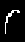
\includegraphics[width=10mm]{w51-r3}}
\subfigure[]{
\includegraphics[width=10mm]{w51-a4}}
\subfigure[]{\includegraphics[width=10mm]{w51-c5}}
\subfigure[]{\includegraphics[width=10mm]{w51-e6}}
\caption{Example of handwritten letter recognition. In the word `brace', the `r' and the `c' look very similar, but can be disambiguated using context. Source: (Taskar et al. 2003) . Used with kind permission of Ben Taskar.}
\end{figure}
\end{frame}

\begin{frame}{Frame Title}
\begin{figure}[h]
\centering
\includegraphics[width=0.5\textwidth]{crfBIO}
\caption{A CRF for joint POS tagging and NP segmentation. Source: Figure 4.E.1 of (Koller and Friedman 2009). Used with kind permission of Daphne Koller.}
\end{figure}    
\end{frame}

\begin{frame}{HMMs for sequences}
\begin{figure}[h]
\centering     %%% not \center
\subfigure[]{\includegraphics[width=40mm]{hmmXY}}
\subfigure[]{\includegraphics[width=40mm]{memmXY}}
\subfigure[]{\includegraphics[width=40mm]{crfXY}}
\caption{Various models for sequential data. (a) A generative directed HMM. (b) A discriminative
directed MEMM. (c) A discriminative undirected CRF.}
\end{figure}

\begin{itemize}
    \item HMM is a generative model of sequences
    \begin{equation}
        p(x, y) =  \prod_{t=1}^T p(y_t |y_{t-1})p(x_t|y_t)
    \end{equation}
    
    \item We cannot easily use global features $x$ (e.g., is the text ALL CAPS), since such features would be ``caused" by all the $y_t$, leading to loss of the Markov property.
    
    \item In addition, even fitting local generative feature models $p(x_t|y_t)$ can be hard.
\end{itemize}
\end{frame}

\begin{frame}{MEMM for sequences}
\begin{itemize}
    \item A maximum entropy Markov model (MEMM) is a discriminative directed model of the form
    \begin{equation}
        p(y|x) =   \prod_t p(y_t |y_{t-1}, x)
    \end{equation}
    
    \item This is easy to train (given labeled data): we just fit a logistic regression (say) model $p(y_t = k|y_{t-1} = j,x)$ separarately for each $k$.
    \item However, it suffers from a subtle problem known as ``label bias".
\end{itemize}
\end{frame}

\begin{frame}{The label bias problem}
\begin{itemize}
    \item The label bias problem is that local features at time $t$ do not influence states prior to time $t$. This follows by examining the DAG, which shows that $x_t$ is d-separated from $y_{t-1}$ (and all earlier time points) by the v-structure at $y_t$, which is a hidden child, thus blocking the information flow.
    \item To understand what this means in practice, consider the part of speech (POS) tagging task. Suppose we see the word ``banks"; this could be a verb (as in ``he banks at BoA"), or a noun (as in ``the river banks were overflowing"). Locally the POS tag for the word is ambiguous. However, suppose that later in the sentence, we see the word ``fishing"; this gives us enough context to infer that the sense of ``banks" is ``river banks". However, in an MEMM (unlike in an HMM and CRF), the ``fishing" evidence will not flow backwards, so we will not be able to disambiguate ``banks". 
\end{itemize}
\end{frame}

\begin{frame}{Skip-chain CRFs for named-entity recognition}
\begin{figure}[h]
\centering
\includegraphics[width=0.7\textwidth]{crfSkip}
\caption{A skip-chain CRF for named entity recognition. Source: Figure 4.E.1 of (Koller and Friedman 2009). Used with kind permission of Daphne Koller.}
\end{figure}

\begin{itemize}
    \item The label space is BIO (begin, inside, other) crossed with Person or Location.
    \item Textually identical strings are likely to correspond to the same state, so we add long-range correlation arcs.
    \item This makes inference more complicated (see later).
\end{itemize}
\end{frame}

\begin{frame}{Discriminative PCFGs}
\begin{figure}[h]
\centering
\includegraphics[width=0.5\textwidth]{altun06-cfg}
\caption{Illustration of a simple parse tree based on a context free grammar in Chomsky normal form. The feature vector $\psi(x, y) = \psi(x, y)$ counts the number of times each production rule was used. Source: Figure 5.2 of (Altun et al. 2006) . Used with kind permission of Yasemin Altun.}
\end{figure}

\begin{itemize}
\item We can define a model of the form
\begin{equation}
    p(y|x) \ \propto \ \exp(w^T \Psi(x, y))
\end{equation}

where $x$ is a sentence, $y$ is a labeled parse tree, and $\Psi(x, y)$ is a feature vector.
\item If $\Psi(x, y)$ factorizes over the parse tree, and the grammar is a probabilistic context free grammar (PCFG), we can compute $\text{arg}\max p(y|x)$ in $O(T^3)$ time using dynamic programming.
\end{itemize}
\end{frame}

                
\subsection{Parameter learning for CRFs}
\begin{frame}{MLE for CRF}
\begin{itemize}
    \item The scaled log-likelihood is
    \begin{equation}
        \begin{split}
            \ell(w) & = \frac{1}{N}\sum_i\log p(y_i|x_i,w)\\
            & = \frac{1}{N}\sum_i\bigg[\sum_c w_c^T\phi_c(y_i,x_i)-\log Z(w,x_i)\bigg] 
        \end{split}
    \end{equation}
    
    \item The gradient is
    \begin{equation}
        \begin{split}
            \frac{\partial\ell}{\partial w_c} & = \frac{1}{N}\sum_i\bigg[\phi_c(y_i,x_i)-\frac{\partial}{\partial w_c}\log Z(w,x_i)\bigg] \\
            & = \frac{1}{N}\sum_i\bigg[\phi_c(y_i,x_i)- E[\phi_c(y,x_i)]\bigg] 
        \end{split}    
    \end{equation}
    
    \item Note that we now have to perform inference for every single training case inside each gradient step, which is $O(N)$ times slower than the MRF case. This is because the partition function depends on the inputs $x_i$.
\end{itemize}
\end{frame}

\begin{frame}{Parameter tying}
\begin{itemize}
    \item In most applications of CRFs (and some applications of MRFs), the size of the graph structure can vary. Hence we need to use parameter tying to ensure we can define a distribution of arbitrary size.
    \item In the pairwise case, we can write the model as follows:
    \begin{equation}
        p(y|x, w) = \frac{1}{Z(w,x)} \exp(w^T \phi(y, x))
    \end{equation}
    
    where $w = [w_n,w_e]$ are the node and edge parameters, and
    \begin{equation}
        \phi(y,x) = [ \sum_t\phi_t(y_t,x), \sum_{s \sim t}\phi_{st}(y_s,y_t,x)]
    \end{equation}
    are the summed node and edge features (these are the sufficient statistics). The gradient expression is easily modified to handle this case.
\end{itemize}
\end{frame}

\begin{frame}{Regularization}
\begin{itemize}
    \item In practice, it is important to use a prior/ regularization to prevent overfitting. If we use a Gaussian prior, the new objective becomes
    \begin{equation}
        \ell'(w) = \frac{1}{N} \sum_i\log p(y_i|x_i,w) - \lambda\|w\|_2^2
    \end{equation}
    It is simple to modify the gradient expression.
    
    \item Alternatively, we can use $\ell_1$ regularization. For example, we could use $\ell_1$ for the edge weights $w_e$ to learn a sparse graph structure, and $\ell_2$ for the node weights $w_n$. In other words, the objective becomes\begin{equation}
        \ell'(w) = \frac{1}{N} \sum_i\log p(y_i|x_i,w) - \lambda_1\|w_e\|_1 - \lambda_2\|w_n\|_2^2
    \end{equation}
    Unfortunately, the optimization algorithms are more complicated when we use $\ell_1$ (see Vishy's tutorial), although the problem is still convex. 
\end{itemize}
\end{frame}

         
\subsection{Structural SVMs, max-margin Markov nets, and all that}
\begin{frame}{Introduction}
\begin{itemize}
    \item SSVMs, M3nets, etc are essentially identical to CRFs The main difference is in the training procedure.
    \item For CRFs, we usually use MAP estimation, i.e., we minimize
    \begin{equation}
        R_{MAP} (w) = - \log p(w) - \sum_{i=1}^N \log p(y_i |x_i , w)
    \end{equation}
    
    \item However, at test time, we pick the label so as to minimize the posterior expected loss:
    \begin{equation}
        \hat{y}(x|w) =\text{arg}\min_{\hat{y}}\sum_y L(y, \hat{y})p(y|x, w)
    \end{equation}
    
    where $L(y^*, \hat{y})$ is the loss we incur when we estimate $\hat{y}$ but the truth is $y^*$.
    \item It therefore seems reasonable to take the loss function into account when performing parameter estimation.
\end{itemize}
\end{frame}

\begin{frame}{A new objective}
\begin{itemize}
    \item Suppose we minimize the (regularized) posterior expected loss on the training set:
    \begin{equation}
        R_{EL}(w) = -\log p(w) + \sum_{i=1}^N \log\bigg[\sum_y L(y_i , y)p(y|x_i , w)\bigg]
    \end{equation}
    
    In the special case of 0-1 loss, $L(y_i , y) = 1 - \delta_{y,y_i}$ , this reduces to RMAP.
    \item Assume that we can write our model in the following form:
    \begin{equation}
        p(y|x, w) = \frac{exp(w^T \phi(x, y))}{z(x,w)}, p(w) = \frac{exp(-E (w))}{Z}
    \end{equation}
    
    where $Z(x,w) = \sum_y \exp(w^T \exp(w^T \phi(x,y))).$
    
    \item Let $L(y_i,y) = \exp\tilde{L}(y_i,y)$.
\end{itemize}
\begin{equation}
    \begin{split}
        R_{EL}(w) & = - \log p(w) + \sum_{i=1}^N \log \bigg[L(y_i, y)p(y|x_i , w)\bigg]\\
        & = -\log p(w) + \sum_i\log \bigg[\sum_y\exp\tilde{L}(y_i,y) \frac{\exp(w^T \phi(x,y))}{Z(x_i,w)}\bigg]\\
        & = E(w) + \sum_i -\log Z(x_i,w) + \log\sum_y \exp(\tilde{L}(y_i,y) + w^T \phi(x,y)) 
    \end{split}
\end{equation}
\end{frame}

\begin{frame}{A convex upper bound}
\begin{itemize}
    \item Using some simple bounds on the log-sum-exp function (see Yuille and He, ``Probabilistic models of vision and max-margin methods", \textit{Frontiers of Electrical and Electronic Engineering} 2011) we can show
    \begin{equation}
        R_{EL}(w)\leq E(w) + \sum_{i=1}^N [\max_y\{\tilde{L}(y_i,y) + w^T \phi(x_i,y)\} - w^T \phi(x_i,y_i) ]
    \end{equation}
    
    \item If we set $E(w)= -\frac{1}{2C} \|w\|_2^2$,
    \begin{equation}
        R_{SSVM}(w) = \frac{1}{2}\|w\|^2 + C\sum_{i=1}^N\bigg[\max_y\{\tilde{L}(y_i,y) + w^T \phi(x_i,y)\} - w^T \phi(x_i,y_i)\bigg]
    \end{equation}
    using loss-augmented decoding.
\end{itemize}
\end{frame}
   
\begin{frame}{The SVM objective}
In the special case that $Y=\{-1,+1\}$ $L(y^*,y)=1-\delta_{y,y^*}$, and $\phi(x, y ) = \frac{1}{2} y x$, this criterion reduces to the following (by considering the two cases that $y = y_i$ and $y \neq y_i$ ):
\begin{equation}
        R_{SVM}(w) = \frac{1}{2}\|w\|^2 + C\sum_{i=1}^N\bigg[\max\{0,1-y_i w^T x_i\}\bigg]
\end{equation}

which is the standard binary SVM objective.
\end{frame}

\begin{frame}{SSVMs vs CRFs}
\begin{itemize}
    \item CRF training and SSVM training are both convex problems (assuming no latent variables).
    \item However, CRF training requires computing marginals $p(y_c|x)$   in the inner loop, whereas SSVM requires computing MAP estimates $\text{arg}\max p(y|x)$. The latter is provably faster in some cases (see later).
    \item In addtion, SSVM training is ``loss aware".
    \item In both cases, the graph structure plays a crucial role in defining the scope of allowable features and enabling efficient inference/ decoding.
\end{itemize}
\end{frame}

\section{Exact inference}
\subsection{Inference}
\begin{frame}{Inferential goals}
\begin{itemize}
    \item Marginals:
    \begin{equation}
        p(x_h|x_v,\theta) = \frac{p(x_h, x_v |\theta)}{p(x_v|\theta)}
    \end{equation}
    
    \item Probability of the evidence:
    \begin{equation}
        p(x_v|\theta) = Z(x_v,\theta) = \sum_{x_h'} p(x_h',x_v|\theta)
    \end{equation}
    
    \item MAP estimation
    \begin{equation}
        \hat{x}_h = \text{arg}\max p(x_h,x_v|\theta)
    \end{equation}
    
    \item Posterior samples $x_h^s \sim p(x_h|x_v, \theta)$.
    \item Inference (often) needed as subroutine for learning $\hat{\theta} = \text{arg}\max p(\theta|D)$.
    \item Can also compute posterior over parameters, $p(\theta|D)$ — Bayesian learning, not covered.
\end{itemize}
\end{frame}

\begin{frame}{Outline of algorithms}
\begin{itemize}
    \item Exact, deterministic.
    \item Approximate, deterministic.
    \item Approximate, stochastic.
\end{itemize}
\end{frame}

\begin{frame}{Types of inference problems for temporal models}
There are different kinds of inference, which we summarize below.
\begin{itemize}
    \item \textbf{} means to compute the \textbf{belief state} $p(z_t|x_{1:t})$ online, or recursively, as the data streams in. This is called ``filtering" because it reduces the noise more than simply estimating the hidden state using just the current estimate, $p(z_t|x_t)$. We will see below that we can perform filtering by simply applying Bayes rule in a sequential fashion. See Figure 24(a) for an example.
    \item \textbf{Smoothing} means to compute $p(z_t|x_{1:T})$ offline, given all the evidence. See Figure 24(b) for an example. By conditioning on past and future data, our uncertainty will be significantly reduced. To understand this intuitively, consider a detective trying to figure out who committed a crime. As he moves through the crime scene, his uncertainty is high until he finds the key clue; then he has an ``aha" moment, his uncertainty is reduced, and all the previously confusing observations are, in hindsight, easy to explain.
\end{itemize}
\end{frame}

\begin{frame}{Frame Title}
\begin{itemize}
    \item \textbf{Fixed lag smoothing} is an interesting compromise between online and offline estimation; it involves computing $p(z_{t-l}|x_{1:t})$, where $l > 0$ is called the \textbf{lag}. This gives better performance than filtering, but incurs a slight delay. By changing the size of the lag, one can trade off accuracy vs delay.
    \item \textbf{Prediction} Instead of predicting the past given the future, as in fixed lag smoothing, we might want to predict the future given the past, i.e., to compute $p(z_{t+h}|x_{1:t})$, where $h > 0$ is called the \textbf{prediction horizon}. For example, suppose $h = 2$; then we have
    \begin{equation}
        p(z_{t+2}|x_{1:t}) = p(z_{t+2} |z_{t+1})p(z_{t+1}|z_t )p(z_t |x_{1:t})
    \end{equation}
    
    It is straightforward to perform this computation: we just power up the transition matrix and apply it to the current belief state. The quantity $p(z_{t+h}|x_{1:t})$ is a prediction about future hidden states; it can be converted into a prediction about future observations using
    
    \begin{equation}
        p(z_{t+h}|x_{1:t}) = p(x_{t+h}|z_{t+h})p(z_{t+h}|x_{1:t})
    \end{equation}
    
    This is the posterior predictive density, and can be used for time-series forecasting (see (Fraser 2008) for details).
\end{itemize}
\end{frame}

\begin{frame}{Frame Title}
\begin{itemize}
    \item \textbf{MAP estimation} This means computing $\text{arg}\max_{z1:T} p(z_{1:T} |x_{1:T})$, which is a most probable state sequence. In the context of HMMs, this is known as \textbf{Viterbi decoding}. Figure 26 illustrates the di erence between filtering, smoothing and MAP decoding for the occasionally dishonest casino HMM. We see that the smoothed (offline) estimate is indeed smoother than the filtered (online) estimate. If we threshold the estimates at 0.5 and compare to the true sequence, we find that the filtered method makes 71 errors out of 300, and the smoothed method makes 49/300; the MAP path makes 60/300 errors. It is not surprising that smoothing makes fewer errors than Viterbi, since the optimal way to minimize bit-error rate is to threshold the posterior marginals. Nevertheless, for some applications, we may prefer the Viterbi decoding.
    \item \textbf{Posterior samples} If there is more than one plausible interpretation of the data, it can be useful to sample from the posterior, $z_{1:T} \sim p(z_{1:T} |x_{1:T})$. These sample paths contain much more information than the sequence of marginals computed by smoothing.
    \item \textbf{Probability of the evidence} We can compute the probability of the evidence, $p(x_{1:T})$, by summing up over all hidden paths, $p(x_{1:T}) = \sum_{z1:T} p(z_{1:T}, x_{1:T})$. This can be used to classify sequences (e.g., if the HMM is used as a class conditional density), for model-based clustering, for anomaly detection, etc. 
\end{itemize}
\end{frame}

\subsection{Forwards-backwards algorithm for chains}
\begin{frame}{Introduction}
\begin{itemize}
    \item Consider a 1d chain representing an HMM 
    \begin{equation}
        p(z, x) = \prod_{t=1}^T p(z_t |z_{t-1})p(x_t |z_t ) 
    \end{equation}
    
    \item We first compute the filtered marginals in the forwards pass 
    \begin{equation}
        \alpha_t(j) = p(z_t = j|x_{1:t})
    \end{equation}
    
    \item We then compute the smoothed marginals in the backwards pass
    \begin{equation}
        \gamma_t(j) p(z_t =j|x_{1:T})
    \end{equation}
    
    \item As we explain below, this forwards-backwards algorithm takes $O(TK^2)$ time. It can also be applied to chain CRFs representing $p(z_{1:T}|x_{1:T})$.
    
    \item A simple modification yields the Viterbi algorithm which computes the most probable sequence of states (not the same as the sequence of most probable states):
    \begin{equation}
        z^* = \text{arg}\max p(z|x_{1:T})
    \end{equation}
\end{itemize}
\end{frame}

\begin{frame}{The occasionally dishonest casino}
\begin{figure}[h]
\centering
\includegraphics[width=0.1\textwidth]{casino}
\caption{An HMM for the occasionally dishonest casino. The blue arrows visualize the state transition diagram $A$. Based on (Durbin et al. 1998, p54).}
\end{figure}

\begin{itemize}
    \item To illustrate the difference between filtering and smoothing, consider the following example from Durbin et al, ``Biological Sequence Analysis: Probabilistic Models of Proteins and Nucleic Acids".
    \item $x_t\in \{1,2,...,6\}$ represents which dice face shows up, and $z_t$ represents the identity of the dice that is being used. Most of the time the casino uses a fair dice, $z = 1$, but occasionally it switches to a loaded dice, $z = 2$, for a short period.
\end{itemize}
\texttt{
Roll: 66415321616211523465321435663426165523423231514246415\\
Dice: LLLLLLLLLLLLLLFFFFFFLLLLLLLLLLLLLLFFFFFFFFFFFFFFFFFFL}
\end{frame}

\begin{frame}{Filtering, smoothing, MAP in the occasionally dishonest casino}
\begin{figure}[h]
\centering     %%% not \center
\subfigure[]{\includegraphics[width=40mm]{hmmCasinoFiltered}}
\subfigure[]{\includegraphics[width=40mm]{hmmCasinoSmoothed}}
\subfigure[]{\includegraphics[width=40mm]{hmmCasinoViterbi}}
\caption{Inference in the dishonest casino. Vertical gray bars denote the samples that we generated using a loaded die. (a) Filtered estimate of probability of using a loaded dice. (b) Smoothed estimates. (c) MAP trajectory. Figure generated by \texttt{casinoDemo}.}
\end{figure}

\begin{itemize}
    \item If we threshold the estimates at 0.5 and compare to the true sequence, we find that the filtered method makes 71 errors out of 300, the smoothed method makes 49/300, and the MAP path makes 60/300 errors.
    \item It is not surprising that smoothing makes fewer errors than Viterbi, since the optimal way to minimize bit-error rate is to threshold the posterior marginals.
    \item Nevertheless, for some applications, we may prefer the Viterbi decoding, to enforce consistency.
\end{itemize}
\end{frame}

\begin{frame}{Kalman filtering and smoothing}
\begin{figure}[h]
\centering     %%% not \center
\subfigure[]{\includegraphics[width=40mm]{kalmanTrackingTruth}}
\subfigure[]{\includegraphics[width=40mm]{kalmanTrackingFiltered}}
\subfigure[]{\includegraphics[width=40mm]{kalmanTrackingSmoothed}}
\caption{Illustration of Kalman filtering and smoothing. (a) Observations (green cirles) are generated by an object moving to the right (true location denoted by black squares). (b) Filtered estimated is shown by dotted red line. Red cross is the posterior mean, blue circles are 95\% confidence ellipses derived from the posterior covariance. For clarity, we only plot the ellipses every other time step. (c) Same as (b), but using offline Kalman smoothing. Figure generated by \texttt{kalmanTrackingDemo}.}
\end{figure}

\begin{itemize}
    \item Suppose $p(z, x)$ is a linear dynamical system subject to Gaussian noise, where $z\in \mathbb{R}^K$ and $x\in \mathbb{R}^D$.
    \item The analog of forwards-backwards is known as \textbf{Kalman filtering/ smoothing}.
\end{itemize}
\end{frame}

\begin{frame}{The forwards algorithm}
We now describe how to recursively compute the filtered marginals, $p(z_t|x_{1:t})$ in an HMM. 

\begin{itemize}
    \item The algorithm has two steps. First comes the prediction step, in which we compute the \textbf{one-step-ahead predictive density;} this acts as the new prior for time $t$:
    \begin{equation}
        (z_t = j|x_{1:t-1}) = \sum_i p(z_t = j |z_{t-1} = i)p(z_{t-1} = i|x_{1:t-1})
    \end{equation}
    
    \item We just apply Bayes rule sequentially to recursively update the belief state:
    \begin{equation}
        \begin{split}
            \alpha_t(j) & = p(z_t = j|x_{1:t}) = p(z_t = j|x_t,x_{1:t-1})\\
            & \ \propto \ p(x_t|z_t = j, \cancel{x_{1:t-1}})p(z_t = j|x_t,x_{1:t-1})
        \end{split}
    \end{equation}
    
    where $p(x_t|z_t = j)$ is the likelihood and the prior is the one-step-ahead predictive density
    \begin{equation}
        p(z_t = j|x_{1:t-1}) = \sum_i p(z_t=j|z_{t-1}=i)\alpha_{t-1}(i)
    \end{equation}
    
    \item This is called the \textbf{predict-update cycle}.
    \item In matrix-vector notation, we can write the update in the following simple form:
    \begin{equation}
        \alpha_t \ \propto \ \psi_t (\Psi^T \odot \alpha_{t-1})
    \end{equation}
    
    \item The base case is $\alpha_1 \ \propto \ \psi_1 \odot \pi$.  See \textbf{hmmFilter} for some Matlab code.
\end{itemize}
\end{frame}

\begin{frame}{The backwards algorithm}
\begin{itemize}
    \item The key decomposition relies on the fact that we can break the chain into two parts, the past and the future, by conditioning on $z_t$:
    \begin{equation}
        \begin{split}
            p(z_t = j|x_{1:T}) & \ \propto \ p(z_t = j,x_{t+1:T}|x_{1:t})\\
            & \propto \ p(z_t = j|x_{1:t})p(x_{t+1:T}|z_t = j, \cancel{x_{1:t}})
        \end{split}
    \end{equation}
    
    where we have defined 
    \begin{equation}
        \beta_t(j) = p(x_{t+1:T}|z_t =j)
    \end{equation}
    
    as the conditional likelihood of future evidence given that the hidden state at time $t$ is $j$.
    (Note that this is not a probability distribution over states, since it does not need to satisfy $\sum_j \beta_t(j) = 1$.) Finally, define
    \begin{equation}
        \gamma_t(j) = p(z_t = j|x_{1:T})
    \end{equation}
    
    as the desired smoothed posterior marginal. From above equation, we have
    \begin{equation}
         \gamma_t(j) = \alpha_t(j)\beta_t(j)
    \end{equation}
    
    \item We now derive a recursive update for $\beta_t$. (It is also possible to directly update $\gamma_t$.)
\end{itemize}
\end{frame}

\begin{frame}{The backwards algorithm}
\begin{itemize}
    \item Working right to left, we have
    \begin{equation}
        \begin{split}
            \beta_{t-1}(i) & = p(x_{t:T}|z_{t-1}=i)\\
            & = \sum_j p(z_t =j,x_t,x_{t+1:T}|z_{t-1} =i)\\
            & = \sum_j p(x_{t+1:T} |z_t =j,\cancel{x_t},\cancel{z_{t-1} =i})p(z_t =j,x_t |z_{t-1} =i)\\
            & = \sum_j p(x_{t+1:T} |z_t =j) p(x_t|z_t=j,\cancel{z_{t-1}=j})p(z_t =j,x_t |z_{t-1} =i)\\
            &  = \sum_j\beta_t(j)\phi_t(j)\phi(i,j)
        \end{split}
    \end{equation}
    
    \item We can write the resulting equation in matrix-vector form as
    \begin{equation}
        \beta_{t-1} = \Psi(\psi_t \odot \beta_t)
    \end{equation}
    
    \item The base case is
    \begin{equation}
        \beta_T(i) = p(x_{T+1:T}|z_T = i) = p(\emptyset|z_T = i) = 1
    \end{equation}
    which is the probability of a non-event.
    
    \item Having computed the forwards and backwards messages, we can combine them to compute $\gamma_t(j) = \alpha_t(j)\beta_t(j)$. The overall algorithm is known as the \textbf{forwards-backwards algorithm}. The pseudo code is very similar to the forwards case; see \texttt{hmmFwdBack} for an implementation. We can think of this algorithm as passing ``messages" from left to right, and then from right to left, and then combining them at each node.
\end{itemize}
\end{frame}

\begin{frame}{The Viterbi algorithm}
\begin{figure}[h]
\centering
\includegraphics[width=0.15\textwidth]{markovTrellis}
\caption{The trellis of states vs time for a Markov chain. Based on (Rabiner 1989).}
\end{figure}

\begin{itemize}
    \item  The Viterbi algorithm can be used to compute the most probable sequence of states in a chain-structured graphical model, i.e., it can compute
    \begin{equation}
        z^* = \text{arg} \max p(z_{1:T} |x_{1:T} )
    \end{equation}
    
    \item  This is equivalent to computing a shortest path through the \textbf{trellis diagram} in Figure 26, where the nodes are possible states at each time step, and the node and edge weights are log probabilities. That is, the weight of a path $z_1,z_2,...,z_T$ is given by
    \begin{equation}
        \log \pi_1(z_1) + \log \phi_1(z_1) +  \sum_{t=2}^T [\log \phi(z_{t-1}, z_t ) + \log \phi_t (z_t )]
    \end{equation}
\end{itemize}
\end{frame}

\begin{frame}{MAP vs MPM}
\begin{itemize}
    \item Before discussing how the algorithm works, let us make one important remark: the (jointly) most probable sequence of states is not necessarily the same as the sequence of (marginally) most probable states.
    \item In Viterbi, when we estimate $z_t$, we ``max out" the other variables:
    \begin{equation}
        z_t^* =\text{arg}\max_{z_t} \max_{z_{1:t -1} ,z_{t +1:T}} p(z_{1:t -1},z_t,z_{t+1:T}|x_{1:T})
    \end{equation}
    
    whereas we when we use forwards-backwards, we sum out the other variables to get a maximum posterior marginal (MPM):
    \begin{equation}
        z_t^* =\text{arg}\max_{z_t} \max_{z_{1:t -1} ,z_{t +1:T}} p(z_{1:t -1},z_t,z_{t+1:T}|x_{1:T})
    \end{equation}
    
    \item The sequence of MPMs may not be equal to the joint MAP sequence, e.g., ``wreck a nice beach" might be the MPM interpretation of a series of acoustic waveforms, but the MAP sequence is more likely to be ``recognize speech".
\end{itemize}
\end{frame}

\begin{frame}{The Viterbi algorithm: forwards pass}
\begin{itemize}
    \item Define the probability of ending up in state $j$ at time $t$, given that we take the most probable path:
    \begin{equation}
        \delta_t(j) =  \max_{z_1,...,z_{t -1}} p(z_{1:t-1}, z_{t} = j|x_{1:t}) 
    \end{equation}
    
    \item The most probable path to state $j$ at time $t$ must consist of the most probable path to some other state $i$ at time $t - 1$, followed by a transition from $i$ to $j$.
    \begin{equation}
        \delta_t(j) = \max_i\delta_{t-1}(i)\psi(i,j)\phi_t(j)
    \end{equation}

    \item We also keep track of the most likely previous state, for each possible state that we end up in:
    \begin{equation}
        a_t(j) = \text{arg}\max\delta_{t-1}(i)\psi(i,j)\psi_t(j)
    \end{equation}
    
    \item
    \begin{equation}
        \delta_1(j) = \pi_j\phi_1(j)
    \end{equation}
\end{itemize}
\end{frame}

\begin{frame}{The Viterbi algorithm: traceback pass (data = C1, C3, C4, C6)}
\begin{figure}[h]
\centering     %%% not \center
\subfigure[]{\includegraphics[width=40mm]{hmmPhone2}}
\subfigure[]{\includegraphics[width=40mm]{viterbi2}}
\caption{Illustration of Viterbi decoding in a simple HMM for speech recognition. (a) A 3-state HMM for a single phone. We are visualizing the state transition diagram. We assume the observations have been vector quantized into 7 possible symbols, $C1,..., C7$. Each state $z_1 , z_2 , z_3$ has a di erent distribution over these symbols. Based on Figure 15.20 of (Russell and Norvig 2002). (b) Illustration of the Viterbi algorithm applied to this model, with data sequence $C1, C3, C4, C6$. The columns represent time, and the rows represent states. An arrow from state i at $t - 1$ to state $j$ at $t$ is annotated with two numbers: the first is the probability of the $i \rightarrow j$ transition, and the second is the probability of generating observation $x_t$ from state $j$. The bold lines/ circles represent the most probable sequence of states. Based on Figure 24.27 of (Russell and Norvig 1995).}
\end{figure}


\begin{itemize}
    \item We start by computing the most probable final state $z_T^*$
    \begin{equation}
        z_T^* =\text{arg}\max\delta_T(i)
    \end{equation}

    \item We can then compute the most probable sequence of states using \textbf{traceback}:
    \begin{equation}
        z_t^* = a_{t+1}(z_{t+1}^*)
    \end{equation}
    
    \item Figure 27 gives a worked example of the Viterbi algorithm, based on (Russell et al. 1995). Suppose we observe the discrete sequence of observations $x_{1:4} = (C1, C3, C4, C6)$, representing codebook entries in a vector-quantized version of a speech signal. The model starts in state $z_1$. The probability of generating $C1$ in $z_1$ is 0.5, so we have $\delta_1(1) = 0.5$, and $\delta_1(i) = 0$ for all other states. Next we can self-transition to $z_1$ with probability 0.3, or transition to z2 with proabability 0.7. If we end up in $z_1$, the probability of generating C3 is 0.3; if we end up in $z_2$,the probability of generating C3 is 0.2. Hence we have
    \begin{equation}
        \begin{split}
            \delta_2(1) & = \delta_1(1)\psi(1, 1)\phi_2(1) = 0.5 \times 0.3 \times 0.3 = 0.045\\
            \delta_2(2) & = \delta_1(1)\psi(1, 2)\phi_2(2) = 0.5 \times 0.7 \times 0.2 = 0.07
        \end{split}
    \end{equation}
    
    Thus state 2 is more probable at $t = 2$; see the second column of Figure 27(b). In time step 3, we see that there are two paths into $z_2$, from $z_1$ and from $z_2$. The bold arrow indicates that the latter is more probable. Hence this is the only one we have to remember. The algorithm continues in this way until we have reached the end of the sequence. One we have reached the end, we can follow the black arrows back to recover the MAP path (which is 1,2,2,3).
\end{itemize}
\end{frame}

\subsection{Belief propagation for trees}
\begin{frame}{Introduction}
\begin{figure}[h]
\centering     %%% not \center
\subfigure[]{\includegraphics[width=10mm]{bptreeUp2}}
\subfigure[]{\includegraphics[width=10mm]{bptreeDown2}}
\caption{Message passing on a tree. (a) Collect-to-root phase. (b) Distribute-from-root phase.}
\end{figure}

\begin{itemize}
    \item Let us assume we have a pairwise MRF or CRF
    \begin{equation}
        p(x|v) = \frac{1}{Z(v)} \prod_{s\in \mathcal{V}} \phi_s(x_s)  \prod_{s,t\in \varepsilon} \phi_{s,t}(x_s,x_t)
    \end{equation}
    
    \item We can send messages from the leaves up to the root and back down to compute posterior marginals $p(x_t|v)$ for each node in $O(VK^2)$ time.
    \item This is a natural generalization of forwards-backwards from chains to trees.
    \item A similar algorithm can be used to compute the MAP estimate or posterior samples.
\end{itemize}
\end{frame}

\begin{frame}{Bottom-up pass}
\begin{itemize}
    \item Goal: compute $\text{bel}_t^- (x_t)= p(x_t|v_t^-)$,
    \item Suppose, by induction, that we have computed ``messages" from $t$'s children: $m_{s\rightarrow t}^-(x_t) = p(x_t|v_{st}^-)$.
    \item Absorb incoming messages from children:
    \begin{equation}
        \text{bel}_t^-(x_t) = p(x_t|v_t^-)=\frac{1}{Z_t}\psi_t(x_t)  \prod_{c\in\text{ch}(t)} m_{c\rightarrow t}^- (x_t)
    \end{equation}
    
    \item Compute message from node s to its parent t:
    \begin{equation}
        m_{s\rightarrow t}^-(x_t) = \sum_{x_s}  \phi_{st} (x_s,x_t)\text{bel}_s^-(x_s)
    \end{equation}
    
    \item Analog of forwards pass.
\end{itemize}
\end{frame}

\begin{frame}{Top-down pass}
\begin{itemize}
    \item Assume we have top-down messages:
    \begin{equation}
        m_{t\rightarrow s}^+ (x_s ) =  p(x_t|v_{st}^+)
    \end{equation}
    
    \item Smoothed posterior belief: absorb all incoming top-down messages
    \begin{equation}
        \text{bel}_s^-(x_s) = p(x_s|v)
        \text{bel}_s^-(x_s)
        \prod_{t\in\text{pa}(s)} m_{t\rightarrow s}^+ (x_s)
    \end{equation}
    
    \item Top-down message (belief updating version):
    \begin{equation}
        m_{t\rightarrow s}^+ (x_s) = p(x_s|v_{st}^+) = \sum_{x_t}\phi_{st}(x_s,x_t)\frac{\text{bel}_t(x_t)}{m_{s\rightarrow t}^- (x_t)}
    \end{equation}
    
    \item Top-down message (sum-product version):
    \begin{equation}
        m_{t\rightarrow s}^+ (x_s) = \sum_{x_t}\phi_{st}(x_s,x_t)\phi_t(x_t)\prod_{c\in\text{ch}(t),c\neq s} m_{c\rightarrow t}^- (x_t)\prod_{p\in\text{pa}(t)} m_{p\rightarrow t}^+ (x_t)
    \end{equation}
    
    \item In the case of a chain, $t$ only has one child $s$ and one parent $p$, so the above simplifies to
    \begin{equation}
        m_{t\rightarrow s}^+ (x_s) = \sum_{x_t}\phi_{st}(x_s,x_t)\phi_t(x_t) m_{p\rightarrow t}^+ (x_t)
    \end{equation}
\end{itemize}
\end{frame}

\begin{frame}{Parallel, distributed version}
\begin{itemize}
    \item We can define a parallel version as follows.
    \item Absorb from all neighbors
    \begin{equation}
        \text{bel}_s^-(x_s) = \phi_s(x_s)\prod_{t\in\text{nbr}_s}m_{t\rightarrow s}(x_s)
    \end{equation}
    
    \item Send messages to each of its neighbors:
    \begin{equation}
        m_{s\rightarrow t} (x_t) = \sum_{x_s}(\phi_s(x_s)\phi_{st}(x_s,x_t)\prod_{u\in\text{nbr}_s\backslash t}m_{u\rightarrow s}(x_s))
    \end{equation}
    
    \item cf systolic array.
    \item Takes $V$ steps to converge for a tree.
    \item For a loopy graph, may not converge, and even if it does, may not be correct (see later).
\end{itemize}
\end{frame}

\subsection{Variable elimination algorithm}
\begin{frame}{Exact inference for general graphs}
\begin{itemize}
    \item What if the graph is not a chain or tree?
    \item We will see that exact inference is exponential in the
    treewidth of the graph, $O(VK^{w+1})$.
    \item For a chain or tree, treewidth is 1, so inference is $O(VK^2)$.
    \item Some graphs have low treewidth, others (eg grids) have large treewidth.
\end{itemize}
\end{frame}

\begin{frame}{Example}
\begin{figure}[h]
\centering     %%% not \center
\subfigure[]{\includegraphics[width=50mm]{student-inf}}
\subfigure[]{\includegraphics[width=50mm]{student-MN}}
\caption{Left: The ``student" DGM. Right: the equivalent UGM. We add moralization arcs D-I, G-J and L-S. Based on Figure 9.8 of (Koller and Friedman 2009).}
\end{figure}
\end{frame}

\begin{frame}{(cont'd)}
\begin{itemize}
    \item Consider the DGM
    \begin{equation}
        P(C,D,I,G,S,L,J,H) = P(C)P(D|C)P(I)P(G|I,D)P(S|I)P(L|G)P(J|L,S)P(H|G,J)
    \end{equation}
    
    \item To convert the DGM to a UGM, we simply define a potential or factor for every CPD, yielding
    \begin{equation}
        p(C,D,I,G,S,L,J,H) = \psi_C(C)\psi_D(D,C)\psi_I(I)\psi_G(G,I,D)\psi_S(S,I)\psi_L(L,G)\psi_J(J,L,S)\psi_H(H,G,J)
    \end{equation}
    \item Suppose we want to compute the prior marginal $p(J)$
\end{itemize}
\end{frame}

\begin{frame}{Variable elimination}
\begin{itemize}
    \item Naively
    \begin{equation}
        p(J) = \sum_J\sum_S\sum_G\sum_H\sum_I\sum_D\sum_C
        p(C,D,I,G,S,L,J,H)
    \end{equation}
    \item We can be smarter by \textbf{pushing sums inside products} (or maxes over sums: generalized distributive law)
\end{itemize}
\end{frame}

\begin{frame}{Graphical representation of Variable elimination}
\begin{figure}[h]
\centering     %%% not \center
\subfigure[]{\includegraphics[width=10mm]{VE-student-steps-a}}
\subfigure[]{\includegraphics[width=10mm]{VE-student-steps-b}}
\subfigure[]{\includegraphics[width=10mm]{VE-student-steps-c}}

\caption{Example of the elimination process, in the order $C$, $D$, $I$, etc. When we eliminate I (figure c), we add a fill-in edge between $G$ and $S$, since they are not connected. Based on Figure 9.10 of (Koller and Friedman 2009).
}
\end{figure}

\begin{itemize}
    \item Every time we eliminate a variable, we add edges to its uneliminated neighbors.
    \item The resulting maximal cliques correspond to the factors created by VE.
    \begin{equation}
        \{C,D\},\{D,I,G\},\{G,L,S,J\},\{G,J,H\},\{G,I,S\}
    \end{equation}
\end{itemize}
\end{frame}

\begin{frame}{Chordal graphs}
\begin{figure}[h]
\centering     %%% not \center
\subfigure[]{\includegraphics[width=20mm]{pentagon}}
\subfigure[]{\includegraphics[width=20mm]{pentagonTriangulated}}

\caption{Left: this graph is not triangulated, despite appearances, since it contains a chordless 5-cycle 1-2-3-4-5-1. Right: one possible triangulation, by adding the 1-3 and 1-4 fill-in edges. Based on (Armstrong 2005, p46)}
\end{figure}

\begin{itemize}
\item The fill-in edges added during VE mean the resulting graph is chordal/ triangulated / chordal.
\item This means that every undirected cycle $X_1 - X_2 ... X_k - X_1$ of length $k \geq 4$ has a chord, i.e., an edge connects $X_i$, $X_j$ for all non-adjacent nodes $i,j$ in the cycle.
\end{itemize}        
\end{frame}

\begin{frame}{Treewidth}
\begin{itemize}
    \item It is clear that the time complexity of VE is
    \begin{equation}
        \prod_{c\in C(G(\prec))}K^{|c|} 
    \end{equation}
    where $C$ are the cliques that are created, $|c|$ is the size of the clique $c$, and we assume for notational simplicity that all the variables have $K$ states each.
    
    \item Let us define the \textbf{induced width} of a graph given elimination ordering $\prec$, denoted $w(\prec)$, as the size of the largest factor (i.e., the largest clique in the induced graph ) minus 1.
    
    \item Then it is easy to see that the complexity of VE with ordering $\prec$ is $O(K^{w(\prec)+1})$.
    
    \item Let us define the treewidth of a graph as the minimal induced width.
    \begin{equation}
        w = min_\prec \max_{c\in G(\prec)} |c|-1
    \end{equation}
    
    Then clearly the best possible running time for VE is $O(DK^{w+1})$.
\end{itemize}
\end{frame}

\begin{frame}{Minimizing treewidth}
\begin{itemize}
    \item  Unfortunately, one can show that for arbitrary graphs, finding an elimination ordering $\prec$ that minimizes $w(\prec)$ is NP-hard.
    \item In practice greedy search techniques are used to find reasonable orderings, although people have tried other heuristic methods for discrete optimization, such as genetic algorithms.
    \item It is also possible to derive approximate algorithms with provable performance guarantees (Amir10).
\end{itemize}
\end{frame}

\subsection{Junction tree algorithm}
\begin{frame}{A weakness of VE}
\begin{itemize}
    \item Consider computing all the marginals in a chain-structured graphical model such as an HMM.
    \item We can easily compute the final marginal $p(x_T |v)$ by eliminating all the nodes $x_1$ to $x_{T-1}$ in order.
    \item This is equivalent to the forwards algorithm, and takes $O(K^2T)$ time.
    \item But now suppose we want to compute $p(x_{T-1}|v)$. We have to run VE again, at a cost of $O(K^2T)$ time. So the total cost to compute all the marginals is $O(K^2T^2)$.
    \item However, we know that we can solve this problem in $O(K^2T)$ using forwards-backwards.
    \item The difference is that FB caches the messages computed on the forwards pass, so it can reuse them later.
\end{itemize}
\end{frame}

\begin{frame}{BP is more efficient}
\begin{figure}[h]
\centering
\includegraphics[width=0.3\textwidth]{treeMsgPassing}
\caption{Sending multiple messages along a tree. (a) $X_1$ is root. (b) $X_2$ is root. (c) $X_4$ is root. (d) All of the messages needed to compute all singleton marginals. Based on Figure 4.3 of (Jordan 2007).}
\end{figure}

\begin{itemize}
    \item VE on a tree is like sending messages to a single root. 
    \item If we re-run it, we are repeating work.
    \item BP is more efficient.
\end{itemize}
\end{frame}

\begin{frame}{Junction trees}
\begin{figure}[h]
\centering     %%% not \center
\includegraphics[width=0.6\textwidth]{koller-9-11}
\caption{(a) The student graph with fill-in edges added. (b) The maximal cliques. (c) The junction tree. An edge between nodes s and $t$ is labeled by the intersection of the sets on nodes s and $t$; this is called the \textbf{separating set}. From Figure 9.11 of (Koller and Friedman 2009). Used with kind permission of Daphne Koller.}
\end{figure}

\begin{itemize}
    \item A junction tree is a tree created from the max cliques of the chordal graph (using some elimination order).
    \item A jtree enjoys the \textbf{running intersection property} (RIP), which means that any subset of nodes containing a given variable forms a connected component.
\end{itemize}
\end{frame}

\begin{frame}{Message passing on a junction tree}
\begin{itemize}
    \item BP on a junction tree will compute the exact values of $p(x_c|v)$ for each node c in the tree (i.e., clique in the induced graph).
    \item From this, we can easily extract the node and edge marginals, $p(x_t|v)$ and $p(x_s,x_t|v)$ from the original model.
    \item The cost is $O(|C|K^{w+1})$, where $w$ is the treewidth.
    \item This generalizes forwards-backwards / BP to arbitrary graphs.
    \item Can also compute MAP estimate and posterior samples.
\end{itemize}
\end{frame}

\subsection{The need for approximate inference}
\begin{frame}{Treewidth can be large}
\begin{figure}[h]
\centering     %%% not \center
\includegraphics[width=0.5\textwidth]{koller-9-1}
\caption{Encoding a 3-SAT problem on n variables and m clauses as a DGM. The $Q_s$ variables are binary random variables. The $C_t$ variables are deterministic functions of the $Q_s$'s, and compute the truth value of each clause. The At nodes are a chain of AND gates, to ensure that the CPT for the final $x$ node has bounded size. The double rings denote nodes with deterministic CPDs. Source: Figure 9.1 of (Koller and Friedman 2009). Used with kind permission of Daphne Koller.}
\end{figure}

 \begin{itemize}
    \item Inference using JTA is exponential in treewidth, but maybe there are better algorithms?
    \item Unlikely since exact inference is \#P-hard (reduction to 3-SAT).
    \item In fact even approximate inference is hard.
 \end{itemize}
 \end{frame}

\begin{frame}{Stochasticity to the rescue}
\begin{itemize}
    \item The hardness results focus on structural (graphical) properties of the model.
    \item Often the edge strengths are weak, so the components are only loosely dependent.
    \item We can exploit this for fast approximate inference.
\end{itemize}
\end{frame}

\end{document}

